%%%%%%%%%%%%%%%%%%%%%%%%%%%%%%%%%%%%%%%%
% datoteka diploma-vzorec.tex
%
% vzorčna datoteka za pisanje diplomskega dela v formatu LaTeX
% na UL Fakulteti za računalništvo in informatiko
%
% vkup spravil Gašper Fijavž, december 2010
% 
%
%
% verzija 12. februar 2014 (besedilo teme, seznam kratic, popravki Gašper Fijavž)
% verzija 10. marec 2014 (redakcijski popravki Zoran Bosnić)
% verzija 11. marec 2014 (redakcijski popravki Gašper Fijavž)
% verzija 15. april 2014 (pdf/a 1b compliance, not really - just claiming, Damjan Cvetan, Gašper Fijavž)
% verzija 23. april 2014 (privzeto cc licenca)
% verzija 16. september 2014 (odmiki strain od roba)
% verzija 28. oktober 2014 (odstranil vpisno številko)
% verija 5. februar 2015 (Literatura v kazalu, online literatura)
% verzija 25. september 2015 (angl. naslov v izjavi o avtorstvu)
% verzija 26. februar 2016 (UL izjava o avtorstvu)
% verzija 16. april 2016 (odstranjena izjava o avtorstvu)
% verzija 5. junij 2016 (Franc Solina dodal vrstice, ki jih je označil s svojim imenom)


\documentclass[a4paper, 12pt]{book}
%\documentclass[a4paper, 12pt, draft]{book}  Nalogo preverite tudi z opcijo draft, ki vam bo pokazala, katere vrstice so predolge!



\usepackage[utf8x]{inputenc}   % omogoča uporabo slovenskih črk kodiranih v formatu UTF-8
\usepackage[slovene,english]{babel}    % naloži, med drugim, slovenske delilne vzorce
\usepackage[pdftex]{graphicx}  % omogoča vlaganje slik različnih formatov
\usepackage{fancyhdr}          % poskrbi, na primer, za glave strani
\usepackage{amssymb}           % dodatni simboli
\usepackage{amsmath}           % eqref, npr.
%\usepackage{hyperxmp}
\usepackage[hyphens]{url}  % dodal Solina
\usepackage{comment}       % dodal Solina

\usepackage{listings}             % Include the listings-package

\usepackage{tikz,wrapfig}
\usepackage{tikz-cd}
\usetikzlibrary{shapes,arrows}
\usetikzlibrary{positioning}

\makeatletter
\renewcommand{\@chapapp}{}% Not necessary...
\newenvironment{chapquote}[2][2em]
  {\setlength{\@tempdima}{#1}%
   \def\chapquote@author{#2}%
   \parshape 1 \@tempdima \dimexpr\textwidth-2\@tempdima\relax%
   \itshape}
  {\par\normalfont\hfill--\ \chapquote@author\hspace*{\@tempdima}\par\bigskip}
\makeatother

\newcommand{\ed}{e^{h\partial}}

\newcommand{\bfW}{\mathbf{W}}
\newcommand{\bfw}{\mathbf{w}}
\newcommand{\bfM}{\mathbf{M}}
\newcommand{\bfm}{\mathbf{m}}
\newcommand{\RR}{\mathbb{R}}
\newcommand{\Ss}{\mathcal{S}}
\newcommand{\II}{\mathbb{I}}
\newcommand{\JJ}{\mathbb{J}}
\newcommand{\E}{\mathcal{E}}
\newcommand{\T}{\mathcal{T}}
\newcommand{\VV}{\mathcal{V}}
\newcommand{\MM}{\mathcal{M}}
\newcommand{\NN}{\mathcal{N}}
\newcommand{\e}{\mathbf{e}}
\newcommand{\x}{\mathbf{x}}
\newcommand{\m}{\mathbf{m}}
\newcommand{\h}{\mathbf{h}}
\newcommand{\uu}{\mathbf{u}}
\newcommand{\vv}{\mathbf{v}}
\newcommand{\F}{\mathcal{F}}
\newcommand{\X}{\mathcal{X}}
\newcommand{\CC}{C\nolinebreak\hspace{-.05em}\raisebox{.4ex}{\tiny\bf +}\nolinebreak\hspace{-.10em}\raisebox{.4ex}{\tiny\bf +}}
\def\CC{{C\nolinebreak[4]\hspace{-.05em}\raisebox{.4ex}{\tiny\bf ++}}}
\newcommand{\dP}{\mathcal{P}}
% operator odvoda
\newcommand{\D}{\partial}
%operator 1 + \D
\newcommand{\DD}{\mathcal{D}}
% operator 1+ \D + \D^2 + ...
\newcommand{\sumd}{\tau}
\DeclareMathOperator{\interior}{int}

\DeclareMathOperator{\proj}{pr}


\usepackage[pdftex, colorlinks=true,
						citecolor=black, filecolor=black, 
						linkcolor=black, urlcolor=black,
						pagebackref=false, 
						pdfproducer={LaTeX}, pdfcreator={LaTeX}, hidelinks]{hyperref}

\usepackage{color}       % dodal Solina
\usepackage{soul}       % dodal Solina

\usepackage{nameref}


%%%%%%%%%%%%%%%%%%%%%%%%%%%%%%%%%%%%%%%%
%	DIPLOMA INFO
%%%%%%%%%%%%%%%%%%%%%%%%%%%%%%%%%%%%%%%%
\newcommand{\ttitle}{Operatorski račun nad programskimi prostori}
\newcommand{\ttitleEn}{Operational Calculus on Programming Spaces}
\newcommand{\tsubject}{\ttitle}
\newcommand{\tsubjectEn}{\ttitleEn}
\newcommand{\tauthor}{Žiga Sajovic}
\newcommand{\tkeywords}{operatorska algebra, tenzorska algebra, nevronske mreže, globoko učenje, avtomatsko odvajanje}
\newcommand{\tkeywordsEn}{operator algebra, tensor algebra, neural networks, deep learning, automatic differentiation}


%%%%%%%%%%%%%%%%%%%%%%%%%%%%%%%%%%%%%%%%
%	HYPERREF SETUP
%%%%%%%%%%%%%%%%%%%%%%%%%%%%%%%%%%%%%%%%
\hypersetup{pdftitle={\ttitle}}
\hypersetup{pdfsubject=\ttitleEn}
\hypersetup{pdfauthor={\tauthor, ziga.sajovic@xlab.si}}
\hypersetup{pdfkeywords=\tkeywordsEn}


 


%%%%%%%%%%%%%%%%%%%%%%%%%%%%%%%%%%%%%%%%
% postavitev strani
%%%%%%%%%%%%%%%%%%%%%%%%%%%%%%%%%%%%%%%%  

\addtolength{\marginparwidth}{-20pt} % robovi za tisk
\addtolength{\oddsidemargin}{40pt}
\addtolength{\evensidemargin}{-40pt}

\renewcommand{\baselinestretch}{1.3} % ustrezen razmik med vrsticami
\setlength{\headheight}{15pt}        % potreben prostor na vrhu
\renewcommand{\chaptermark}[1]%
{\markboth{\MakeUppercase{\thechapter.\ #1}}{}} \renewcommand{\sectionmark}[1]%
{\markright{\MakeUppercase{\thesection.\ #1}}} \renewcommand{\headrulewidth}{0.5pt} \renewcommand{\footrulewidth}{0pt}
\fancyhf{}
\fancyhead[LE,RO]{\sl \thepage} 
%\fancyhead[LO]{\sl \rightmark} \fancyhead[RE]{\sl \leftmark}
\fancyhead[RE]{\sc \tauthor}              % dodal Solina
\fancyhead[LO]{\sc Diplomska naloga}     % dodal Solina


\newcommand{\BibTeX}{{\sc Bib}\TeX}

%%%%%%%%%%%%%%%%%%%%%%%%%%%%%%%%%%%%%%%%
% naslovi
%%%%%%%%%%%%%%%%%%%%%%%%%%%%%%%
\newcommand{\autfont}{\Large}
\newcommand{\titfont}{\LARGE\bf}
\newcommand{\clearemptydoublepage}{\newpage{\pagestyle{empty}\cleardoublepage}}
\setcounter{tocdepth}{1}	      % globina kazala

%%%%%%%%%%%%%%%%%%%%%%%%%%%%%%%%%%%%%%%%
% konstrukti
%%%%%%%%%%%%%%%%%%%%%%%%%%%%%%%%%%%%%%%%  
\newtheorem{posledica}{Posledica}[chapter]
\newtheorem{izrek}{Izrek}[chapter]
\newtheorem{opomba}{Opomba}[chapter]
\newtheorem{lemma}{Lemma}[chapter]
\newtheorem{definicija}{Definicija}[chapter]
\newtheorem{trditev}{Trditev}[izrek]
\newenvironment{dokaz}{\emph{Dokaz.}\ }{\hspace{\fill}{$\Box$}}

%%%%%%%%%%%%%%%%%%%%%%%%%%%%%%%%%%%%%%%%%%%%%%%%%%%%%%%%%%%%%%%%%%%%%%%%%%%%%%%
%% PDF-A
%%%%%%%%%%%%%%%%%%%%%%%%%%%%%%%%%%%%%%%%%%%%%%%%%%%%%%%%%%%%%%%%%%%%%%%%%%%%%%%


%%%%%%%%%%%%%%%%%%%%%%%%%%%%%%%%%%%%%%%% 
% define medatata
%%%%%%%%%%%%%%%%%%%%%%%%%%%%%%%%%%%%%%%% 
\def\Title{\ttitle}
\def\Author{\tauthor, ziga.sajovic@xlab.si}
\def\Subject{\ttitleEn}
\def\Keywords{\tkeywordsEn}

%%%%%%%%%%%%%%%%%%%%%%%%%%%%%%%%%%%%%%%% 
% \convertDate converts D:20080419103507+02'00' to 2008-04-19T10:35:07+02:00
%%%%%%%%%%%%%%%%%%%%%%%%%%%%%%%%%%%%%%%% 
\def\convertDate{%
    \getYear
}

{\catcode`\D=12
 \gdef\getYear D:#1#2#3#4{\edef\xYear{#1#2#3#4}\getMonth}
}
\def\getMonth#1#2{\edef\xMonth{#1#2}\getDay}
\def\getDay#1#2{\edef\xDay{#1#2}\getHour}
\def\getHour#1#2{\edef\xHour{#1#2}\getMin}
\def\getMin#1#2{\edef\xMin{#1#2}\getSec}
\def\getSec#1#2{\edef\xSec{#1#2}\getTZh}
\def\getTZh +#1#2{\edef\xTZh{#1#2}\getTZm}
\def\getTZm '#1#2'{%
    \edef\xTZm{#1#2}%
    \edef\convDate{\xYear-\xMonth-\xDay T\xHour:\xMin:\xSec+\xTZh:\xTZm}%
}

\expandafter\convertDate\pdfcreationdate 

%%%%%%%%%%%%%%%%%%%%%%%%%%%%%%%%%%%%%%%%
% get pdftex version string
%%%%%%%%%%%%%%%%%%%%%%%%%%%%%%%%%%%%%%%% 
\newcount\countA
\countA=\pdftexversion
\advance \countA by -100
\def\pdftexVersionStr{pdfTeX-1.\the\countA.\pdftexrevision}


%%%%%%%%%%%%%%%%%%%%%%%%%%%%%%%%%%%%%%%%
% XMP data
%%%%%%%%%%%%%%%%%%%%%%%%%%%%%%%%%%%%%%%%  
\usepackage{xmpincl}
\includexmp{pdfa-1b}

%%%%%%%%%%%%%%%%%%%%%%%%%%%%%%%%%%%%%%%%
% pdfInfo
%%%%%%%%%%%%%%%%%%%%%%%%%%%%%%%%%%%%%%%%  
\pdfinfo{%
    /Title    (\ttitle)
    /Author   (\tauthor, ziga.sajovic@xlab.si)
    /Subject  (\ttitleEn)
    /Keywords (\tkeywordsEn)
    /ModDate  (\pdfcreationdate)
    /Trapped  /False
}


%%%%%%%%%%%%%%%%%%%%%%%%%%%%%%%%%%%%%%%%%%%%%%%%%%%%%%%%%%%%%%%%%%%%%%%%%%%%%%%
%%%%%%%%%%%%%%%%%%%%%%%%%%%%%%%%%%%%%%%%%%%%%%%%%%%%%%%%%%%%%%%%%%%%%%%%%%%%%%%

\newcommand{\CcImageCc}[1]{%
	
\includegraphics[scale=#1]{license/cc_cc_30.pdf}%
}
\newcommand{\CcImageBy}[1]{%
	
\includegraphics[scale=#1]{license/cc_by_30.pdf}%
}
\newcommand{\CcImageSa}[1]{%
	
\includegraphics[scale=#1]{license/cc_sa_30.pdf}%
}

\begin{document}
\selectlanguage{slovene}
\frontmatter
\setcounter{page}{1} %
\renewcommand{\thepage}{}       % preprecimo težave s številkami strani v kazalu
\newcommand{\sn}[1]{"`#1"'}                    % dodal Solina (slovenski narekovaji)

%%%%%%%%%%%%%%%%%%%%%%%%%%%%%%%%%%%%%%%%
%naslovnica
 \thispagestyle{empty}%
   \begin{center}
    {\large\sc Univerza v Ljubljani\\%
      Fakulteta za računalništvo in informatiko}%
    \vskip 10em%
    {\autfont \tauthor\par}%
    {\titfont \ttitle \par}%
    {\vskip 3em \textsc{DIPLOMSKO DELO\\[5mm]         % dodal Solina za ostale študijske programe
%    VISOKOŠOLSKI STROKOVNI ŠTUDIJSKI PROGRAM\\ PRVE STOPNJE\\ RAČUNALNIŠTVO IN INFORMATIKA}\par}%
    UNIVERZITETNI  ŠTUDIJSKI PROGRAM\\ PRVE STOPNJE\\ RAČUNALNIŠTVO IN INFORMATIKA}\par}%
%    INTERDISCIPLINARNI UNIVERZITETNI\\ ŠTUDIJSKI PROGRAM PRVE STOPNJE\\ RAČUNALNIŠTVO IN MATEMATIKA}\par}%
%    INTERDISCIPLINARNI UNIVERZITETNI\\ ŠTUDIJSKI PROGRAM PRVE STOPNJE\\ UPRAVNA INFORMATIKA}\par}%
%    INTERDISCIPLINARNI UNIVERZITETNI\\ ŠTUDIJSKI PROGRAM PRVE STOPNJE\\ MULTIMEDIJA}\par}%
    \vfill\null%
    {\large \textsc{Mentor}: prof.\ dr.  Borut Robič\par}%
    {\vskip 2em \large Ljubljana, 2017 \par}%
\end{center}
% prazna stran
%\clearemptydoublepage      % dodal Solina (izjava o licencah itd. se izpiše na hrbtni strani naslovnice)

%%%%%%%%%%%%%%%%%%%%%%%%%%%%%%%%%%%%%%%%
%copyright stran
\thispagestyle{empty}
\vspace*{8cm}

\noindent
{\sc Copyright}. 
{\small \noindent
To delo je ponujeno pod licenco \textit{Creative Commons Priznanje avtorstva-Deljenje pod enakimi pogoji 2.5 Slovenija} (ali novej\v so razli\v cico).
To pomeni, da se tako besedilo, slike, grafi in druge sestavine dela, kot tudi izvorna koda lahko prosto distribuirajo,
reproducirajo, uporabljajo, priobčujejo javnosti in predelujejo, pod pogojem, da se jasno in vidno navede avtorja in naslov tega
dela in da se v primeru spremembe, preoblikovanja ali uporabe tega dela v svojem delu, lahko distribuira predelava le pod
licenco, ki je enaka tej.
Podrobnosti licence so dostopne na spletni strani \href{http://creativecommons.si}{creativecommons.si} ali na Inštitutu za
intelektualno lastnino, Streliška 1, 1000 Ljubljana.

\begin{center}% 0.66 / 0.89 = 0.741573033707865
\CcImageCc{0.741573033707865}\hspace*{1ex}\CcImageBy{1}\hspace*{1ex}\CcImageSa{1}%
\end{center}
}

% prazna stran
\clearemptydoublepage

%%%%%%%%%%%%%%%%%%%%%%%%%%%%%%%%%%%%%%%%
% stran 3 med uvodnimi listi
\thispagestyle{empty}
\vspace*{4cm}

\noindent
Fakulteta za računalništvo in informatiko izdaja naslednjo nalogo:
\medskip
\begin{tabbing}
\hspace{32mm}\= \hspace{6cm} \= \kill




Tematika naloge:
\end{tabbing}
Razvijte algebraični jezik, ki bo deloval kot formalni račun za globoko učenje, hkrati pa bo orodje za proučevanje programov, ki so v njem implementirani. Jezik naj deluje kot poln model globokega učenja. Omogoča naj tako izražanje programov, da bo že njihov zapis nudil teoretični vpogled vanje.
\vspace{15mm}






\vspace{2cm}

% prazna stran
\clearemptydoublepage

% zahvala
\thispagestyle{empty}\mbox{}\vfill\null\it%
\noindent
Avtor se zahvaljuje Mariu Medvedu podjetja XLAB za vero in podporo pri razvoju ubesedene teorije, Martinu Vuku za potrpežljivost ob izraznih izomorfizmih, Jure Kališniku za preverbo dokazov in Borutu Robiču za vodstvo skozi akademsko življenje.
\rm\normalfont

% prazna stran
\clearemptydoublepage

%%%%%%%%%%%%%%%%%%%%%%%%%%%%%%%%%%%%%%%%
% posvetilo, če sama zahvala ne zadošča :-)
\thispagestyle{empty}\mbox{}{\vskip0.20\textheight}\mbox{}\hfill\begin{minipage}{0.55\textwidth}%
Za Barbi.
\normalfont\end{minipage}

% prazna stran
\clearemptydoublepage


%%%%%%%%%%%%%%%%%%%%%%%%%%%%%%%%%%%%%%%%
% kazalo
\pagestyle{empty}
\def\thepage{}% preprecimo tezave s stevilkami strani v kazalu
\tableofcontents{}


% prazna stran
\clearemptydoublepage

%%%%%%%%%%%%%%%%%%%%%%%%%%%%%%%%%%%%%%%%
% povzetek
\addcontentsline{toc}{chapter}{Povzetek}
\chapter*{Povzetek}

\noindent\textbf{Naslov:} \ttitle
\bigskip

\noindent\textbf{Avtor:} \tauthor
\bigskip

%\noindent\textbf{Povzetek:} 
\noindent
V delu razvijemo algebraični jezik, ki predstavlja formalen račun za globoko učenje, in je hkrati model, v katerem je programe mogoče tako implementirati kot tudi preučevati.

V ta namen razvijemo abstrakten \emph{računski model avtomatsko odvedljivih programov}. V njem so programi elementi t.i. \emph{programskih prostorov}. Programe gledamo kot preslikave končno-dimenzionalnega vektorskega prostora vase, imenovanega \emph{navidezni pomnilniški prostor}. Navidezni pomnilniški prostor je algebra programov, torej \emph{algebraična podatkovna struktura} (s katero je mogoče računati). Elementi navideznega pomnilniškega prostora pa omogočajo razvoj programov v neskončne tenzorske vrste. Na programskih prostorih definiramo \emph{operator odvajanja}, s pomočjo njegovih potenc pa implementiramo \emph{posplošen operator premika} in \emph{operator kompozicije} programov.

Tako konstruiran algebraični jezik je poln model globokega učenja. Omogoča tak način izražanja programov, da že njihov zapis nudi teoretični vpogled vanje.

\bigskip

\noindent\textbf{Ključne besede:} \tkeywords.
% prazna stran
\clearemptydoublepage

%%%%%%%%%%%%%%%%%%%%%%%%%%%%%%%%%%%%%%%%
% abstract
\selectlanguage{english}
\addcontentsline{toc}{chapter}{Abstract}
\chapter*{Abstract}

\noindent\textbf{Title:} \ttitleEn
\bigskip

\noindent\textbf{Author:} \tauthor
\bigskip

%\noindent\textbf{Abstract:} 
\noindent 
In this work we develop an algebraic language, that represents a formal calculus for deep learning and is, at the same time, a model that enables implementations and investigations of programs.

To this purpose we develop an \emph{abstract computational model of automatically differentiable programs}. In it, programs are elements of op. cit. \emph{programming spaces}. Programs are viewed as maps on a finite-dimensional vector space, to itself op. cit. \emph{virtual memory space}. Virtual memory space is an algebra of programs, \emph{an algebraic data structure} (one can calculate with). The elements of the virtual memory space give the expansion of programs into an infinite tensor series. We define a \emph{differential operator} on programming spaces and implement the \emph{general shift operator} and the \emph{operator of program composition} in terms of its powers.

An algebraic language constructed in this way is a complete model of deep learning. It enables us to express programs in such a way, that their properties may be derived from their source codes.

\bigskip

\noindent\textbf{Keywords:} \tkeywordsEn.
\selectlanguage{slovene}
% prazna stran
\clearemptydoublepage

%%%%%%%%%%%%%%%%%%%%%%%%%%%%%%%%%%%%%%%%
\mainmatter
\setcounter{page}{1}
\pagestyle{fancy}

\chapter{Uvod}

Zaradi diskretne narave računalniške znanosti prihaja do vrzeli med matematično analizo in programiranjem. Medtem ko se je algebra že vpletla v veje programiranja preko algebraičnih podatkovnih tipov funkcijskih jezikov, njena uporaba ostaja predvsem v problemih, ki so diskretni in kombinatorični. A zaradi hitrosti razvoja strojnega in globokega učenja se pojavlja potreba po modelih programiranja, ki bi omogočali obravnavo (odskoma) zveznih in odvedljivih programskih struktur \cite{AdSurvey}. Tej potrebi delno že zadoščajo sodobne metode avtomatskega odvajanja. Te metode omogočajo učinkovit izračun odvodov matematičnih funkcij implementiranih v obliki računalniških programov \cite{AD1}. Vendar pa ne omogočajo algebraičnega manipulacija s programi in tako tudi ne vplivajo na bistvo polemike o razkolu (ki je v nezmožnosti algebraičnega manipulacija odvedljivih programov).

Namen tega dela je zapolniti vrzel med programiranjem in analizo, ki je značilno za trenutno stanje \cite{AD2}. 

V drugem poglavju (\emph{\nameref{ch:MotivacijaInOzadje}}) bomo predstavili, kako lahko \emph{delno} prevedemo \emph{algebraične podatkovne tipe} funkcijskih jezikov (kot npr. Haskell) v vsote in produkte elementov neke algebraične strukture. Razgalili bomo probleme v teh jezikih, ki so razlog, da je prevajanje le \emph{delno}. Izpostavili bomo tudi slabost \emph{globokega učenja}, kjer zaradi pomanjkanja formalnega aparata obravnava poteka predvsem empirično in s tem utemeljili potrebo po rezultatih našega dela. Opisali bomo tudi pomena našega dela za področje \emph{avtomatskega odvajanja} programov, ki je v splošni uporabi v uporabnem računalništvu (npr. v inženiringu, simulacijah).

V tretjem poglavju (\emph{\nameref{ch:programskiProstori}}) pričnemo z vzpostavitvijo potrebnih objektov za konstrukcijo takega algebraičnega jezika. Programe interpretiramo kot preslikave vektorskih prostorov vase in na podlagi take interpretacije definiramo \emph{avtomatsko odvedljive programe}. 

Naš računski model razširimo v četrtem poglavju (\emph{\nameref{ch:OdvProgPros}}), ko konstruiramo \emph{navidezni pomnilniški prostor}. Slednji deluje kot \emph{algebraična podatkovna struktura}, tj. podatkovna struktura, s katero se da računati. Tako podatkovno strukturo potrebujemo za konstrukcijo t.i. \emph{odvedljivih programskih prostorov}, katere strogo definiramo in dokažemo potrebne izreke o njihovi zaprtosti. Poglavje zaključimo z definicijo \emph{navideznih tenzorskih strojev}, ki konstruirajo odvedljive programske prostore, in z \emph{implementacijo} odvedljive različice jezika $\CC$, ki je dostopna na avtorjevi GitHub strani \cite{dC++}.

V petem poglavju (\emph{\nameref{ch:opRac}}) na podlagi prej vpeljanih programskih prostorov razvijemo algebraični jezik, ki deluje kot formalni račun globokega učenja in je hkrati model, v katerem je programe mogoče tako implementirati kot tudi preučevati. Nato izpeljemo splošen \emph{razvoj programov v tenzorsko vrsto}, ter izpeljemo še operatorja \emph{premika} in \emph{kompozicije} programov. Slednja omogočata konstrukcijo iteratorjev in komponerjev. Pokažemo, kako vsi ti operatorji delujejo kot abstrakcije, ki omogočajo, da se izračune opravi samo z operatorji preden te apliciramo na konkreten program - s tem se izognemo delu s tenzorskimi vrstami. 
Nato razvijemo preslikavo redukcije reda in s tem rešimo problem gnezdenega odvajanja \cite{AD2}, saj omogoča implementacije programov, ki operirajo na odvedljivimi odvodi drugih programov.
Z vpeljanimi operatorji pokažemo, da naša teorija uvaja poln (samozadosten) model globokega učenja. Ta model omogoča tak način izražanja programov, da že njihov zapis razgalja njihove lastnosti. Poglavje zaključimo z obravnavo pomena naše teorije za kontrolne strukture ter z napotki za uporabo teorije v praksi.

Diplomsko delo temelji na avtorjevih člankih \cite{opCalProg} \cite{dC++Paper} in delu \cite{dC++}\cite{dC++Man}, kamor bralca usmerimo v zaključnem poglavju (\emph{\nameref{ch:zakSklp}}), v katerem navedemo možnosti, ki jih izpeljana teorija še ponuja.

\chapter{Motivacija in ozadje}
\label{ch:MotivacijaInOzadje}

\begin{chapquote}{\small{John Backus, \textit{Can Programming Be Liberated From the von Neumann Style?}}}
``Von Neumann languages do not have useful properties for reasoning about programs. Axiomatic and denotational semantics are precise tools for describing and understanding conventional programs, but they only talk about them and cannot alter their ungainly properties. Unlike von Neumann languages, the language of ordinary algebra is suitable both for stating its laws and for transforming an equation into its solution, all within the language.''
\end{chapquote}

Po prejetju Turingovega nagrade leta 1977 za delo na prevajalniku za programski jezik Fortran je imel John Backus svoje slavno predavanje, kot nekakšno opravičilo za svoje delo. Namreč, v predavanju je kritiziral von Neumannove jezike (katerih predstavnik je ravno Fortran), kot tudi von Neumannovo računalniško arhitekturo. Toda segel je še globlje in se obregnil ob neobstoj nekakšne algebre programov, ki bi programskim jezikom omogočala, da bi sklepali o programih, katere implementirajo \cite{backus}.
V prihodnjih letih je računalniška znanost pričela z raziskavami Backusoih skrbi. Njegovo skrb glede zaporednega izvajanja, tj. von Neumannovega ozkega grla, dodobra naslavljajo nedavni napredki na področju strojne opreme in arhitekture, ki danes streže tudi globokem učenju (npr. Nvidia, Google TPU). Vendar njegova skrb algebraičnega obravnavanja programov še vedno tli. Jeziki, kot je Haskell, implementirajo algebraične podatkovne tipe s pomočjo teorije kategorij. Povezavo takih podatkovnih tipov s klasično algebro, ter njihove pomanjkljivosti bomo spoznali v razdelku \ref{algTp}.

Globoko učenje je programska paradigma, ki zaradi svoje algebraične naravnanosti ponuja možnost formalizma, ki naslavlja obe Backusovi skrbi. Trenutno je globokega učenja še vedno v pomanjkanju formalizma, zato večinoma temelji na empiričnih spoznanjih. Področje bomo na kratko spoznali v razdelku \ref{sec:deepLearning} in izpostavili to pomanjkanje formalizma.
Razvoj algebraičnega jezika, ki vsebuje globoko učenje, je plod avtorjevega dela zadnjih let \cite{opCalProg} \cite{dC++Paper}. Ker je področje prežeto z gradienti in Jacobiani, je področje soočeno s potrebo po jeziku, ki bi omogočal sklepanje o analitičnih lastnostih programov zgolj z uporabo algebraičnih prijemov. Kot bomo videli, tej potrebi lahko zadostimo z uporabo tenzorske algebre in operatorskega računa, predstavljenega v našem delu.
Tak formalizem pa je tudi orodje, ki presega globoko učenje in teoretična preučevanja programskih jezikov, saj vsebuje posplošitev in poenotenje metod avtomatskega odvajanja (razdelek \ref{sec:avtOdv}).

\section{Algebra algebraičnih podatkovnih tipov}\label{algTp}

Predmet tega razdelka je algebra algebraičnih podatkovnih tipov ter njene lastnosti in pomanjkljivosti, ki jih bomo za lažje razumevanje prikazali na primeru Haskella. Slednje je povzeto po zapisih \cite{algTip}.

V splošnem je algebrska struktura množica objektov ter operacij nad njimi, ki omogočajo transformacije teh objektov v nove objekte. V algebri tipov jezika Haskell so objekti podatkovni tipi, denimo \emph{Bool} in \emph{Int}, operacije pa gradijo iz danih tipov nove, kompleksnejše tipe. Primer je konstruktor \emph{Either}, ki izgradi nov tip \emph{Either Bool Int} iz tipov Bool in Int.

\subsection{Operacije}

\subsubsection{Preštevanje}

Povezavo z algebro števil lahko vzpostavimo s preštevanjem možnih vrednosti, ki jih tip lahko zasede. Na primeru \emph{Bool}, definiranim z
$$data\text{ }Bool = False\text{ }\vert \text{ }True,$$
to pomeni, da lahko tip \emph{Bool} zasede dve vrednosti. (Lahko bi zasedel tudi \emph{undefined}, a tej vrednosti se v prid razlagi izognemo). Tako prispemo do nove definicije.
\begin{definicija}[Izomorfnost tipov]\label{def:iso}
Izomorfnost ($===$) dveh tipov $Type_1$ in $Type_2$ definiramo s
$$Type_1===Type_2 \iff \vert Type_1\vert = \vert Type_2\vert,$$
kjer $\vert Type\vert$ označuje število vrednosti, ki jih tip lahko zaseda.
\end{definicija}
Če sta dva tipa izomorfna po definiciji \ref{def:iso}, med njima obstaja bijektivna preslikava. Na zgornjem primeru to pomeni
$$Bool === 2,$$
kar bomo podrobneje razjasnili, ko bomo spoznali aditivne tipe.

Če je \emph{Bool} enak $2$, čemu je enaka $1$? V literaturi so takšni objekti navadno poimenovani z \emph{Unit}; v Haskell je Unit označen z \emph{()}.

\subsubsection{Vsota}

Če sta $a$ in $b$ tipa, potem je tip $Add\text{ }a\text{ }b$, ki ustreza njuni vsoti, definiran z
$$data\text{ }Add\text{ }a\text{ }b=AddL\text{ }a\text{ }|\text{ }AddR\text{ }b.$$
Torej, tip $Add\text{ }a\text{ }b$ je oblika unije\footnote{ang. tagged union}, ki vsebuje bodisi $a$ ali $b$. Zakaj tip $Add\text{ }a\text{ }b$ ustreza vsoti $a+b$ tipov $a$ in $b$ je razvidno iz preštevanja. Na primer, tip $Add\text{ }Bool\text{ }()$ vsebuje $\vert Bool\vert+\vert ()\vert=2+1=3$ vrednosti. V Haskellu je tipu $Add\text{ }a\text{ }b$ izomorfen tip \emph{Either a b}, a v našem delu je primernejše poimenovanje \emph{Add}.

\subsubsection{Produkt}

Če sta $a$ in $b$ tipa, potem je tip $Mul\text{ }a\text{ }b$, ki ustreza njunemu produktu, definiran z
$$data\text{ }Mul\text{ }a\text{ }b=Mul\text{ }a\text{ }b.$$
Torej, tip $Mul\text{ }a\text{ }b$ je zbirnik, ki drži tako $a$, kot $b$. Zakaj tip $Mul\text{ }a\text{ }b$ ustreza produktu $a\cdot b$ tipov $a$ in $b$ je razvidno iz preštevanja. Na primer, $Mul\text{ }Bool\text{ }Bool$ vsebuje $\vert Bool\vert\cdot\vert Bool\vert=2\cdot 2=4$ vrednosti.  V Haskellu je tipu $Mul\text{ }a\text{ }b$ izomorfen tip \emph{(a.b)}, a v našem delu je primernejše poimenovanje \emph{Mul}.

\subsubsection{Ničla - identiteta za operacijo vsote}

Z vsoto in produktom lahko iz tipa \emph{Unit} generiramo tipe, ki ustrezajo pozitivnim celim številom. Še vedno pa manjka tip, ki bi ustrezal številu $0$, torej tip brez vrednosti. Tak tip definiramo z
$$data\text{ \emph{Void}}.$$
Ker definicija ne vsebuje konstruktorja, vrednosti tipa \emph{Void} ni mogoče konstruirati - to pomeni, da ima \emph{nič} vrednosti.

\subsection{Zakoni v algebri tipov}

Kakor v algebri števil, tudi v algebri tipov zakoni določajo enakost dveh objektov (po definiciji enakosti \ref{def:iso}). V prid jasnosti navajamo primer implementacije izomorfizma
$$Bool===Add\text{ }()\text{ } (),$$
ki jo vidimo na sliki \ref{code:iso}.

\begin{figure}\label{code:iso}
\lstset{language=Haskell}
\begin{lstlisting}[frame=single]
to :: Bool -> Add () ()
to False = AddL ()
to True  = AddR ()

from :: Add () () -> Bool
from (AddL _) = False
from (AddR _) = True
\end{lstlisting}
\caption{Primer izomorfizma}
\end{figure}

\subsubsection{Zakoni vsote tipov}

Navajamo primer dveh zakonov vsote tipov. 

\noindent Prvi veli
$$Add\text{ \emph{Void}}\text{ \emph{a}}===\text{\emph{a}},$$
da ima tip \emph{Add Void a} toliko vrednosti, kot tip \emph{a}. 

\noindent Drugi veli
$$Add\text{ }a\text{ }b===Add\text{ }b\text{ }a,$$
da je vrstni red operandov nepomemben. 

\noindent Oba zakona sta bralcu verjetno bolj poznana iz algebre števil, kjer se glasita
$$0+a=a,$$
ter
$$a+b=b+a.$$
Zakona za algebro tipov bi lahko dokazali s konstrukcijo, kot je bilo storjeno na sliki \ref{code:iso}, a to prepuščamo bralcu.

\subsubsection{Zakoni produkta tipov}

Navajamo tri koristne zakone, ki se nanašajo na produkt tipov. 

\noindent Prvi veli
$$Mul\text{ \emph{Void}}\text{ }a===\text{\emph{Void}},$$
da je produkt poljubnega tipa s tipom \emph{Void} enak tipu \emph{Void}, kar je moč interpretirati na sledeč način: ker je nemogoče konstruirati objekt tipa \emph{Void}, je nemogoče konstruirati urejen par tipov, ki bi vseboval tip \emph{Void}. 

\noindent Drugi zakon veli
$$Mul\text{ }()\text{ }a===a,$$
da je toliko urejenih parov, ki imajo tip \emph{Unit} na prvem mestu, kot je vrednosti tipa \emph{a}, ki je na drugem mestu.

\noindent Tretji zakon veli
$$Mul\text{ }a\text{ }b===Mul\text{ }b\text{ }a,$$
da je število urejenih parov dveh tipov enako, ne glede na vrstni red tipov. Ti zakoni so bralcu verjetno bolj poznani iz algebre števil, kjer se glasijo
\begin{eqnarray}
0\cdot a&=&0,\\
1\cdot a&=&a,\\
a\cdot b&=&b\cdot a.
\end{eqnarray}
Iz zgornjih zakonov algebre tipov je možno izpeljati tudi druge zakone, ki jih poznamo iz algebre števil, denimo zakon distributivnosti
$$Mul\text{ }a\text{ }(Add\text{ }b\text{ }c)===Add\text{ }(Mul\text{ }a\text{ }b)\text{ }(Mul\text{ }a\text{ }c),$$
oziroma
$$a\cdot(b+c)=a\cdot b+a\cdot c.$$

\subsection{Funkcijski tipi}

Ob konkretnih tipih, kot sta \emph{Int} in \emph{Bool}, poznamo tudi funkcijske tipe, denimo \emph{Int $\to$ Bool}. V algebro tipov jih umestimo preko preštevanja. Koliko funkcij tipa \emph{a $\to$ b} obstaja? Za pojasnitev navajamo primer. Vzemimo tip s tremi vrednostmi,
$$data\text{ }Trio=prvi\text{ }\vert\text{ } drugi\text{ }\vert\text{ } tretji,$$
ter preštejmo vse funkcije tipa
$$Trio\to Bool.$$
Po kratkem razmisleku je očitno, da je teh funkcij $\vert Bool\vert^{\vert Trio\vert}=2^3=8$, oziroma v splošnem
$$\vert B^A\vert=\vert B\vert^{\vert A\vert},$$
kjer $B^A$ označuje množico vseh funkcij tipa $A\to B$.

\subsubsection{Zakoni funkcijskih tipov}

Obstajata dva zakona funkcijskih tipov, ki vključujeta enoto (\emph{Unit}). 

\noindent Prvi veli
$$()\to a===a,$$
da je toliko funkcij tipa \emph{()$\to$a}, kot je vrednosti tipa \emph{a}.

\noindent Drugi veli
$$a\to ()=== (),$$
da obstaja natanko ena funkcija tipa \emph{a $\to$ ()}; označimo jo z \emph{const ()}. 

\noindent V algebri števil sta to zakona
$$a^1=a,$$
ter
$$1^a=1.$$
Obstaja pa tudi zakon, ki dovoljuje faktorizacijo skupnih argumentov. Označimo z $(a\to b, a\to c)$ urejen par dveh funkcijskih tipov $a\to b$ in $a\to c$. Potem zakon pravi
$$(a\to b, a\to c)===a\to(b,c),$$
kjer $a\to(b,c)$ označuje funkcijski tip, ki slika iz $a$ v urejen par $(b,c)$. V algebri števil je ustrezni zakon
$$b^a\cdot c^a=(b\cdot c)^a.$$
Obstaja pa tudi zakon o funkcijah, ki vračajo funkcije:
$$a\to (b\to c)===(b,a)\to c,$$
katerega oblika v algebri števil je
$$(c^b)^a=c^{b\cdot a}.$$

\subsection{Rekurzivni tipi}

V prejšnjem razdelku smo vpeljali operacije nad tipov ter navedli njihove osnovne lastnosti. S tem smo vzpostavili algebro tipov. V tem razdelku pokažemo dvoje: najprej uporabe algebre tipov nad kompleksnejšimi tipi, potem pa izpostavimo pomanjkljivosti, ki jih zaznamo v tej algebri.

\subsubsection{Seznami}

Ena od osnovnejših struktur večine programskih jezikov je \emph{seznam}. Seznam \emph{L a} objektov tipa \emph{a} je bodisi prazen (\emph{None}), ali pa je sestavljen iz objekta tipa \emph{a}, ki je pripet na obstoječ seznam tipa \emph{a}. To rekurzivno (induktivno) definicijo na kratko izrazimo z
\begin{equation}
data\text{ }L\text{ }a=None\text{ }\vert\text{ } a\text{ }(L\text{ }a). \label{eq:listHaskell}
\end{equation}

V algebri tipov vpeljani v prejšnjih razdelkih, seznam izrazimo kot
$$L(a)=1+a\cdot L(a).$$
Enačbo lahko pričnemo razvijati, kjer bomo izraze tipa $a\cdot a$ nadomestili z $a^2$:
\begin{eqnarray}
L(a)&=& 1+a\cdot L(a)\label{eq:list}\nonumber \\
L(a)&=& 1+a\cdot(1+a\cdot L(a))\nonumber\\
L(a)&=& 1+a+a^2\cdot(1+a\cdot L(a))\nonumber\\
L(a)&=& 1+a+a^2+a^3+\cdots. \label{eq:listEnd}
\end{eqnarray}
Izraz \eqref{eq:listEnd} pravi da obstaja natanko en prazen seznam (člen $1$), natanko en seznam z enim elementom (člen $a$), natanko en seznam z dvema elementoma (člen $a^2$), itd.

Poznavanje rodovnih funkcij in formalnih potenčnih vrst nam (skupaj z zakoni prejšnjega razdelka) omogoča tudi drug način kodiranja informacije zapisane v izrazu \eqref{eq:listHaskell}:
$$L(a)=1+a\cdot L(a)$$
$$\implies$$
\begin{equation}
L(a)=\frac{1}{1-a}\label{eq:listE}
\end{equation}
$$\implies$$
$$L(a)=\sum\limits_{i=0}^\infty a^i,$$
kar je identično dognanje kot rekurzivni razvoj v \eqref{eq:listEnd}. Tukaj poudarimo, da so algebraične manipulacije v \eqref{eq:listE} dovoljene, saj gre le za drug način kodiranja iste informacije. Pri splošnih algebraičnih manipulacijah tipov, kjer z manipuliranjem enakosti izražamo nove enakosti (ne le druge oblike začetnih enakosti) lahko naletimo na težave; to bomo spoznali v razdelku \ref{ch:algMani}.

\subsubsection{Dvojiška drevesa}

V gramatiki jezika Haskell je dvojiško drevo \emph{T} z vrednostmi v vozliščih:
\begin{equation}\label{eq:binT}
data\text{ }T\text{ } a = None \text{ }|\text{ } Node\text{ } a\text{ } (T\text{ } a)\text{ }(T\text{ }a)
\end{equation}

V naši algebri tipov izraz \eqref{eq:binT} postane vsota dveh tipov: tipa \emph{None}, ki je ekvivalenten (po definiciji \ref{def:iso}) tipu \emph{()}, in produkta tipov. Tokrat gre za produkt \emph{treh} tipov, vendar je ta le gnezden produkt \emph{(a, (b, c))}.

V naši algebri tipov izraz \eqref{eq:binT} zapišemo kot
\begin{equation}
\label{eq:binTe}
T(a)=1+a\cdot T(a)^2,
\end{equation}
torej z kvadratno enačbo \eqref{eq:binTe}. Do njene rešitve bi se lahko dokopali podobno kot v računu \eqref{eq:list} s substitucijo, a poskusimo lahko tudi z algebro tipov, kot smo storili v računu \eqref{eq:listE}. Tedaj je rešitev kvadratne enačbe \eqref{eq:binTe}
\begin{equation}
T(a)=\frac{1-\sqrt{1-4\cdot a}}{2\cdot a}, \label{eq:binTeQ}
\end{equation}
izraz, ki ga spet razumemo le kot način kodiranja informacije, in ki ga razčlenimo v Taylorjevo vrsto
\begin{equation}
T(a)=1\cdot a^0+1\cdot a+2\cdot a^2 + 5\cdot a^3+ 14\cdot a^4 + 42\cdot a^5\cdots \label{eq:binExp}
\end{equation}
Zadnji izraz nam daje informacijo, da obstaja: \emph{eno prazno} binarno drevo (člen $1\cdot a^0$), \emph{eno} binarno drevo \emph{s po enim vozliščem} (člen $1\cdot a$), \emph{dve} binarni drevesi \emph{s po dvema vozliščema} (člen $2\cdot a^2$), \emph{pet} binarnih dreves \emph{s po tremi vozlišči} (člen $5\cdot a^3$), $\dots$, kot je prikazano na sliki \ref{fig:trees} in tudi v \cite{analComb}.
\begin{figure}
\begin{center}
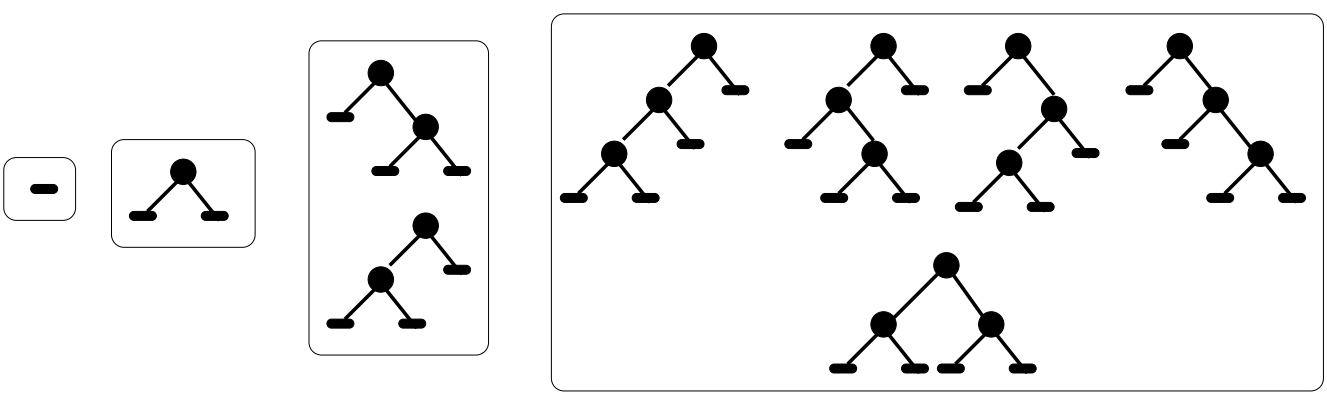
\includegraphics[width=\linewidth]{imgs/bintrees.png}
\end{center}
\caption{Binarna drevesa}
\label{fig:trees}
\end{figure}

Izraz \eqref{eq:binExp} torej prešteva različne vrste dvojiških dreves. Ta lastnost preštevanja nam je poznana iz kombinatoričnih rodov (ang. combinatiorial species) \cite{species}. Vendar \emph{rodovi} niso isto kot tipi; če enakosti s tipi brezskrbno manipuliramo, lahko naletimo na težave, kot bomo spoznali v naslednjem razdelku \ref{ch:algMani}.


\subsection{Algebraične manipulacije}\label{ch:algMani}

Namen algebraičnega manipuliranja enakosti je, da bi izpeljali nova spoznanja. Vprašanje pa je, ali lahko s tipi računamo tako svobodno kot smo vajeni iz algebre števil, ne pa le da neko enakost izrazimo v drugi obliki, kot smo enakost \eqref{eq:binTe} izrazili kot \eqref{eq:binTeQ}. Odgovor je ne, razlogi pa sledeči.

Zaradi neobstoja negativnih tipov, gre v primeru algebraičnih podatkovnih tipov za polkolobar (tj. kolobar brez inverzov). Zato moramo poznati podrobnosti ustreznih algebrskih struktur, da vemo, katere algebraične manipulacije na tipih so legalne (in kdaj). Vemo naslednje \cite{complexCat}: 

\noindent Če pričnemo z enakostjo med kompleksnim številom $t\in\mathbb{C}$ in poljubnim polinomom $p(t)$ s kompleksnimi koeficienti
$$t=p(t),$$
in jo z algebraičnimi manipulacijami razvijemo v
$$q_1(t)=q_2(t),$$
kjer $q_1$ in $q_2$ nista konstanti, potem so te manipulacije legalne tudi v kateremkoli polkolobarju. To pomeni, da je rezultat legalen tudi za algebraične podatkovne tipe (saj ti tvorijo polkolobar) in da obstaja postopek, ki nas pripelje do identičnega rezultata brez uporabe inverzov (tj. deljenja in odštevanja).

Navedimo dva primera algebraičnih manipulacij. Iz enakosti \eqref{eq:binTe} lahko z manipulacijami razvijemo enakost
$$T(a)^7=T(a),$$
ki veli, da je sedmerec dvojiških dreves izomorfen enemu samem dvojiškem drevesu. Na prvi pogled to ni posebno globok rezultat, saj sta obe množici števno neskončni. A obstaja eksplicitna bijekcija med množicama, kot je pokazano v \cite{7Trees}, kjer  avtor pokaže, da za bijekcijo ni potrebno gledat globlje od štirih nivojev drevesa. Rezultat algebraičnih manipulacij je veljaven (legalen), saj obstaja izpeljava brez uporabe inverzov.
A če obe strani enačbe delimo s $T$ pridemo do enakosti
$$T(a)^6=1,$$
ki veli, da je šesterec dvojiških dreves izomorfen enoti (tj. \emph{Unit}). To pa je očiten nesmisel in manipulacij ni mogoče predrugačiti v takšne, ki ne bi vsebovale inverzov.

Skozi naštete razloge vidimo veliko pomanjkljivost algebre algebraičnih tipov: 
\emph{pri manipuliranju z enakostmi zahteva dobro poznavanje zakonitosti algebrskih struktur}. Zato se bomo s tretjim poglavjem (\nameref{ch:programskiProstori}) lotili konstrukcije modela, ki bo vseboval inverze in zato omogočal algebraične manipulacije, kot jih je bralec vajen iz algebre števil. Model bo slonel na paradigmi globokega učenja, ki jo spoznamo v naslednjem razdelku \ref{sec:deepLearning}.


\section{Globoko učenje in pomanjkanje formalizma}\label{sec:deepLearning}

Globoko učenje je uporaba umetnih nevronskih mrež za učenje nalog. Nevronska mreža je definirana z rekurzivno enačbo
$$L^{i+1}=\phi_i(W_i\cdot L^i +b_i),$$
kjer je $L^i$ izhod $i$-tega nivoja, $W_i$ in $b_i$ sta uteži in pristranost (ang. bias), operacija $\cdot$ pa bilinearna operacija (kot denimo tenzorska kontrakcija, ali pa konvolucija), $\phi_i$ pa aktivacijska (ne-linearna) funkcija. Obstaja množica različnih arhitektur \cite{ConvNet}\cite{LSTM}\cite{resNet}, katere so polne po Turingu, če omogočajo rekurzijo \cite{DLbook}. V zadnjih letih se je globoko učenje izkazalo na široki paleti problemov, od prepoznave slik \cite{fasterRCNN}, sledenja \cite{trackNet}, generiranje besedil, govora in slik \cite{genText}, obravnavanja naravnega jezika \cite{NLP}, itd.

Globoko učenje temelji na multilinearnih transformacijah, ki se dajo zlahka paralelizirati (prva od Backusovih skrbi), kar s pridom izkoriščamo za implementacije na GPU \cite{TensorGPU}. Multilinearne transformacije lahko opišemo s tenzorsko algebro. To sicer omogoča algebraične manipulacije, a potrebni formalizem še ne obstaja v polni obliki \cite{whyDL}.

\subsection{Pomanjkanje formalizma}

Globoko učenje je izrazljivo s tenzorsko algebro, a sklepanje o implementiranih modelih še vedno poteka v (matematičnem) jeziku, ki je ločen od implementacijskega jezika. Pravzaprav odsotnost formalizma sega tako daleč, da dandanes še ni natančne definicije globokega učenja.
Leon Buttou, spoštovan strokovnjak s področja globokega učenja, je v korespondenci z avtorjem dejal:

\begin{chapquote}{\small{dr. Leon Buttou, \textit{V korespondenci z avtorjem}}}
``\dots There is no proper definition of what deep learning even is at this stage. Your [avtorjeva] theory of Operational Calculus on Programming Spaces \cite{opCalProg} could offer a first such definition through the formalism you [avtor] propose.''
\end{chapquote}

Snovanje tega manjkajočega formalizma je predmet našega dela. Konstruirali bomo algebraični jezik, ki predstavlja poln model globokega učenja. Z izpeljanim formalizmom bomo predlagali in prikazali nov način izražanja programov ter kako ta način uporabiti za izpeljavo novih arhitektur globokega učenja v teoretično utemeljenem kontekstu.

\section{Tenzorska algebra}\label{sec:tenAlg}

Tenzorska algebra vektorskega prostora $V$, ki jo označimo z $T(V)$, je algebra tenzorjev na $V$, pri kateri je bilinearna preslikava tenzorski produkt. Je prosta algebra (ang. free algebra) na $V$, in hkrati najsplošnejša algebra, ki vsebuje $V$, v smislu korespondence na univerzalno lastnost \cite{tenCalc1}.
Tenzorska algebra je pomembna, saj porodi mnoge algebre, kot kvocientne algebre $T(V)$, kar bomo s pridom izkoristili.

\subsection{Univerzalna lastnost}

Tenzorska algebra zadošča sledeči univerzalni lastnosti, ki formalno izraža izjavo, da je najsplošnejša algebra, ki vsebuje $V$.

Vsaka linearna transformacija $f:V\to A$, iz $V$ v algebro $A$ nad poljem $K$, je lahko enkratno razširjena na algebro morfizmov iz $T(V)$ v $A$, kot je prikazano na sledečem komutativnem diagramu
\begin{equation*}
\begin{tikzcd}
V \arrow{r}{i}  \arrow{rd}{f} 
  & T(V) \arrow[dashed]{d}{\tilde{f}} \\
    & A
\end{tikzcd}
\end{equation*}
kjer je $i$ kanonična vključitev $V$ v $T(V)$. Definiramo lahko tenzorsko algebro $T(V)$ kot edino algebro, ki zadošča tej lastnosti, a kljub temu moramo pokazati, da tak objekt res obstaja \cite{tenCalc2}.

\subsection{Kvocienti}

Zaradi splošnosti tenzorske algebre, je mnoge druge algebre mogoče konstruirati tako, da pričnemo s tenzorsko algebro, v katero vpeljemo določene relacije nad generatorji, tj. konstruiramo določene kvocientne algebre $T(V)$. Primer tega je simetrična algebra, ki jo bomo uporabili tudi v tem delu.

\section{Avtomatsko odvajanje}\label{sec:avtOdv}

Avtomatsko odvajanje je množica tehnik za izračun odvodov funkcij, ki so implementirane kot računalniški programi. Izkorišča dejstvo, da vsak program, ne glede na svojo kompleksnost sestoji iz izvršitev osnovnih operacij in funkcij. Tehnike omogočajo učinkovite izračune odvodov, v $\mathcal{O}(1)$-krat daljšem času \cite{AdSurvey}.

\subsection{Vnaprejšnji in vzvratni način avtomatskega odvajanja}

Temelj avtomatskega odvajanja je dekompozicija diferencialov s pomočjo verižnega pravila. Navadno sta predstavljeni dva načina avtomatskega odvajanja. \emph{Vnaprejšnji način} \cite{PcAD} in \emph{vzvratni način} \cite{ReverseAD} avtomatskega odvajanja. Vnaprejšnji način določa obiskovanje verižnega pravila od navznoter proti navzven, medtem ko vzvratni način določa obisk od navzven proti navznoter.

V splošnem, sta obe obliki specifična primera uporabe operatorja kompozicije programov, ki ga izpeljemo v tem delu (glej razdelek \ref{sec:OpKompo}) in s tem avtomatsko odvajanje dvignemo iz učinkovitega načina izračuna odvodov, v algebraično orodje.

\chapter{Programski prostori} \label{ch:programskiProstori}

\section{Programi kot Preslikave vektorskih prostorov}\label{sec:progKotPres}

Programe bomo modelirali, kot preslikave vektorskih prostorov. Če se osredotočimo na spremenljivke, ki zasedajo realne vrednosti (tj. tipa float ali double) je stanje pomnilnika predstavljivo z visoko dimenzionalnim vektorjem. Množica vseh možnih spominskih stanj je lahko modelirana s končno dimenzionalnim vektorskim prostorom $\VV\simeq\RR^n$ (podobno kot pri Nevronskih Turingovih strojih \cite{neuTur}). Prostor $\VV$ bomo poimenovali \emph{pomnilniški prostor programa}. Akcija programa nad svojim pomnilniškim prostorom je opisljiva z
\begin{equation}
P:\VV\to\VV
\end{equation}
Programski prostor je prostor preslikav $\VV\to\VV$, ki so lahko implementirane kot program v programskem jeziku.
\begin{definicija}[Evklidski stroj]
Dvojec $(\VV,\F)$ je Evklidski stroj, kjer
\begin{itemize}
\item
$\VV$ je končno dimenzionalen vektorski prostor, nad poljem $K$, ki služi kot pomnilnik
\item
$\F<\VV^\VV$ je podprostor preslikav $\VV\to\VV$, ki služi kot akcije nad pomnilnikom.
\end{itemize}
\end{definicija}

Na prvi pogled se Evklidski stroj zdi kot opis funkcijskega programiranja, s kompozicijami podedovanimi od $\F$. Nameren vtis, saj želimo da naša konstrukcija premore lastnosti funkcijskega programiranja. S tem namenom predpostavljamo standarden model nad $\F$, kjer je odvedljivost edini dodatni pogoj, ki ga vsilimo s prihajajočimi razdelki.

\section{Odvedljive preslikave in programi}

Pred definiranjem odvedljivih programov, se spomnimo nekaj definicij.
\begin{definicija}[Odvod]
Naj bosta $V,U$ Banachova prostora. Preslikava $P:V\to U$ je odvedljiva v točki
  $\x\in V$, če obstaja omejen linearen operator $TP_\x:V\to U$ kjer
  \begin{equation}
    \label{eq:frechet}
    \lim_{\h\to 0}\frac{\|P(\x+\h)-P(\x)-TP_\x(\h)\|}{\|\h\|} = 0.
  \end{equation}
  Preslikava $TP_\x$ je imenovana \emph{Fréchet odvod} preslikave $P$ v točki $\x$.
\end{definicija}

Za preslikave $\RR^n\to\RR^m$ je Fréchet odvod izrazljiv kot množenje vektorja $\h$ z matriko $\mathbf{J}_{P,\x}$ parcialnih odvodov komponent preslikave $P$
\begin{equation*}
  T_\x P(\h) = \mathbf{J}_{P,\x}\cdot \h.
\end{equation*}

V preostanku tega razdelka predvidevamo, da je preslikava $P:V\to U$ odvedljiva za vse $\x\in V$. Odvod definira preslikavo iz $V$ v omejene linearne preslikave iz $V$ v $U$. Predpostavljamo tudi, da sta $V$ in $U$ končno dimenzionalna. Potem je prostor linearnih preslikav iz $V$ v $U$ izomorfen tenzorskem produktu $U\otimes V^*$, kjer je izomorfizem dan skozi tenzorske kontrakcije, in pošlje preprost tenzor $\uu\otimes f\in U\otimes V^*$ v linearno preslikavo
\begin{equation}
   \label{eq:lin_tenzor}
   \uu\otimes f:\x \mapsto f(\x)\cdot \uu.
 \end{equation}
Odvod definira preslikavo
\begin{eqnarray}
  \label{eq:odvod_preslikava}
  \D P&:& V\to U\otimes V^*\\
  \D P&:& \x \mapsto T_\x P.
\end{eqnarray}
Obravnavamo pa lahko tudi odvedljivost odvoda samega $\D P$, kar vodi do višjih odvodov.
\begin{definicija}[Višji odvodi]
Naj bo $P:V\to U$ preslikava iz vektorskega prostora $V$ v vektorski prostor $U$. Odvod $\D^k P$ reda $k$ preslikave $P$ je preslikava
\begin{eqnarray}\label{eq:partial}
    \label{eq:visji_odvod}
    \D^kP&:&V\to U\otimes (V^*)^{\otimes k}\\
    \D^kP&:&\x\mapsto T_\x\left( \D^{k-1}P \right)
  \end{eqnarray}
\end{definicija}
\begin{opomba}
V zgornji definiciji predpostavljamo, da je preslikava $P$, kot tudi vsi odvodi, odvedljiva za vse točke $\x$. V kolikor temu ni tako, je zgornje definicije mogoče izrazit lokalno, kar bi vpeljalo v večini tehnične težave.
\end{opomba}
Naj bo  $\e_1,\ldots,\e_n$ baza prostora $U$ in $x_1,\ldots x_m$ baza prostora $V^*$. Z $P_i=x_i\circ P$ označimo $i$-to komponento preslikave $P$ glede na bazo $\{e_i\}$ prostora $U$. Potem je $\D^k P$ lahko definiran skozi smerne (parcialne) odvode s formulo
\begin{equation}\label{eq:d}
	\partial^kP=\sum_{\forall_{i,\alpha}}\frac{\partial^k P_i}{\partial
	    x_{\alpha_1}\ldots \partial x_{\alpha_k}}\e_i\otimes
	  dx_{\alpha_1}\otimes\ldots \otimes dx_{\alpha_k}.
\end{equation}

\section{Odvedljivi programi}

Želimo si sposobnost, da bi predstavili odvode programov v Evklidskem stroju kot programe v istem Evklidskem stroju. S tem namenom bomo definirali tri podporstore v pomnilniškem prostoru $\VV$, ki opisujejo kako različni deli pomnilnika vplivajo na končen rezultat programa.

Označimo z $\e_1,\ldots \e_n$ standardno bazo pomnilniškega prostora $\VV$, in z $x_1,\ldots x_n$ dualno bazo $\VV^*$. Funkcije $x_i$ so koordinatne funkcije na $\VV$ in ustrezajo posamičnim lokacijam (spremenljivkam) v pomnilniku programa.
\begin{definicija}
Za vsak program $P$ v programskem prostoru $\F<\VV^\VV$, definiramo vhodni prostor oziroma prostor parametrov $I_P<\VV$ in zunanji prostor $O_P<\VV$, kot minimalen vektorski podprostor, ki ga napenja standardna baza, kjer je preslikava $P_e$ definirana skozi sledeč komutativen diagram
\begin{equation} 
    \label{eq:induced_map}
\begin{tikzcd}
  \VV \arrow{r}{P} & 
  \VV \arrow{d}{\mathrm{pr}_{O_P}}\\
  I_P \arrow[hook]{u}{\vec{i}\mapsto \vec{i}+\vec{f}} 
  \arrow{r}{P_e}& O_P
\end{tikzcd}
  \end{equation}
ki je neodvisen od izbire elementa $\vec{f}\in F_P=(I_P+O_P)^\perp$.

Prostor $F_P=(I_P+O_P)^\perp$ poimenujemo prost prostor programa $P$.
\end{definicija}

Spremenljivke $x_i$, ki ustrezajo standardni bazi vektorjev in napenjajo parametre, izhode in prost prostor, so imenovane \emph{vhodne spremenljivke}, \emph{izhodne spremenljivke} in \emph{proste spremenljivke}. \emph{Proste spremenljivke} so tiste, ki ostajajo nedotaknjene s strani programa in nimajo vpliva na končen rezultat. Izhod programa je odvisen zgolj od vrednosti vhodnih spremenljivk in sestoji iz spremenljivk katerih vrednosti so bile spremenjene tekom izvajanja programa. Vhodne in izhodne spremenljivke imajo lahko neprazen presek.

Preslikava $P_e$ je imenovana \emph{akcijska preslikava programa} $P$ in opisuje dejansko akcijo programa $P$ nad svojim pomnilniškim prostorom, in ignorira prost pomnilnik.

Odvod akcijske preslikave je predmet interesa, ko govorimo o odvedljivosti programov.
\begin{definicija}[Avtomatsko odvedljivi programi]\label{def:autDef}
Program $P_\VV\to\VV$ je avtomatsko odvedljiv, če obstaja vložitev prostora $O_P\otimes I_P^*$ v prost prostor $F_P$ in tak program $(1+\D )P:\VV\to \VV\oplus(\VV\otimes\VV^*)$, da je njegova akcijska preslikava
\begin{equation}
    \label{eq:program_derivative}
    P_e\oplus \D P_e:I_P\rightarrow O_P\oplus (O_P\otimes I^*).
  \end{equation}
Program $P:\VV\to\VV$ je avtomatsko odvedljiv do reda $k$, če obstaja program $\sumd_k P:\VV\to \VV$, kjer je akcijska preslikava
\begin{equation}
    \label{eq:program_derivative_higher}
    P_e\oplus \D P_e\oplus \ldots \D^k P_e:I_P\rightarrow O_P\oplus \left(O_P\otimes I^*\right)\oplus\ldots \left( O_P\otimes \left( I_p^*\right)^{k\otimes} \right).
  \end{equation}
\end{definicija}

Če je program $P:\VV\to\VV$ avtomatsko odvedljiv, potem je tudi odvedljiv kot preslikava $\VV\to\VV$. Ampak samo odvod akcijske preslikave programa $P$ lahko implementiramo kot program, saj je v praksi pomnilniški prostor omejen na $\VV$, da pa lahko odvajamo program do $k$-te stopnje, moramo izračunat in hranit vse odvode reda $k$ in manj.

\chapter{Odvedljivi programski prostori} \label{ch:OdvProgPros}

Pomnilniški prostor programa je redko obravnavan kot kaj več kot zgolj shramba. A da obdarimo Evklidski stroj z dodano strukturo, ravno sem uperimo svoj pogled. Ohlapno rečeno, je funkcijsko programiranje opisano skozi monoide (grupe brez inverzov), zato se (multi)linearno algebraičen opis pomnilnika zdi primeren korak k pridobitvi dodatne strukture.

\section{Virtualni pomnilniški prostor}

Motivirani z Definicijo \ref{def:autDef}, definiramo pomnilniški prostor programov kot zaporedje vektorskih prostorov po sledeči rekurzivni formuli:
\begin{eqnarray}
  \VV_0 &=& \VV\\
  \label{eq:universal_space}
  \VV_k &=& \VV_{k-1}+\left(\VV_{k-1}\otimes \VV^*\right).
\end{eqnarray}
Poudarjamo, da vsota ni direktna, saj so nekateri podprostori $\VV_{k-1}$ in $\VV_{k-1}\otimes\VV^*$ izomorfni in bodo identificirani drug z drugim.

Prostor, ki zadošča rekurzivni formuli \eqref{eq:universal_space} je
\begin{equation}
    \label{eq:k-th-virtual-space}
    \VV_k = \VV\otimes \left(K\oplus \VV^* \oplus (\VV^*\otimes \VV^*)\oplus\ldots
      (\VV^*)^{\otimes k}\right) = \VV\otimes T_k(\VV^*),
  \end{equation}
kjer je $T_k(\VV^*)$ podprostor tenzorske algebre $T(\VV^*)$, ki sestoji iz linearnih kombinacij tenzorjev ranga $k$ ali manj. Ta konstrukcija nam omogoča, da definiramo vse odvode kot preslikave z isto domeno in ko-domeno $\VV\to\VV\otimes T(V^*)$.

Kot tak je virtualni pomnilniški prostor preslikava iz sebe vase
\begin{equation}
\VV_n:\VV\to\VV,
\end{equation}
kjer je za $W\in\VV_n$ definirana kot 
\begin{equation}
\bfW(\vv)=\bfw_0+\bfw_1\cdot\vv+\cdots+\bfw_n\cdot(\vv)^{\otimes n}\label{eq:Contraction}
\end{equation}
vsota večih kontrakcij (kjer so $\bfw_i\in\VV_i$). Enakost \eqref{eq:Contraction} bomo strogo definirali v razdelku \ref{sec:vrsta}. S takšno konstrukcijo razširitve in kontrakcije pomnilniškega prostora, spominjajoč na dihanje sklada, dobijo pomen izven zgolj hranjenja, kar motivira novo definicijo.
\begin{definicija}[Navidezni pomnilniški prostor]
Naj bo dvojec $(\VV,\F)$ Evklidski stroj in
\begin{equation}
\VV_\infty = \VV\otimes T(\VV^*) = \VV\oplus
(\VV\otimes\VV^*)\oplus\ldots,\label{eq:virtual-memory}
\end{equation}
kjer je $T(\VV^*)$ tenzorska algebra dualnega prostora $\VV^*$. Potem $\VV_\infty$ poimenujemo navidezni pomnilniški prostor Evklidskega stroja $(\VV,\F)$.
\end{definicija}
Izraz navidezen pomnilnik je uporabljen, saj je mogoče vložit le omejeno število podprostorov $\VV_\infty$ v pomnilniški prostor $\VV$, s čimer je pristop podoben pristopu navideznega pomnilnika.

Vsak program $P:\VV\to\VV$ lahko razširimo na preslikavo navideznim pomnilniškim prostorom $\VV_\infty$, tako da nastavimo prvo komponento direktne vsote \eqref{eq:virtual-memory} na $P$, ostale komponente pa na $0$. Podobno lahko odvode $\D^k P$ obravnavamo kot preslikave iz $\VV$ v $\VV_\infty$, tako da nastavimo $k$-to komponento direktne vsote \eqref{eq:virtual-memory} na $\D^k P$, ostale pa na $0$.

\section{Odvedljivi programski prostori}

Za jasnost izražanja definiramo sledeče funkcijske prostore:
 \begin{equation}\label{eq:F_n}
 	\F_n=\{f:\VV\to \VV\otimes T_n(\VV^*)\}
 \end{equation}
Ti funkcijski prostori so lahko videni kot podprostori $\F_\infty=\{f:\VV\to \VV\otimes
T(\VV^*)\}$, saj je $\VV$ naravno vložen v $\VV\otimes T(\VV^*)$. Fréchetov odvod definira operator na prostoru gladkih preslikav $\F_\infty$ \footnote{Operator $\D$ je delno lahko definiran tudi za druge preslikave, a več o tem kasneje.}. Slika katerekoli preslikave $P:\VV\to\VV$ operatorja $\D$ je njen prvi odvod, višji odvodi pa so kar potence operatorja $\D$ aplicirane na $P$. Tako je $\D^k$ preslikava med funkcijskimi prostori \eqref{eq:F_n}
\begin{equation}\label{eq:toFn+k}
 \D^k:\F^n\to\F^{n+k}.
 \end{equation}
\begin{definicija}[Odvedljiv programski prostor]
Odvedljiv programski prostor $\dP_0$ je vsak podprostor $\F_0$, kjer
\begin{equation}\label{eq:P}
 	\D\dP_0\subset\dP_0\otimes T(\VV^*)
\end{equation}
Prostor $\dP_n<\F_n$, ki ga napenja $\{\D^k\dP_0;\quad 0\le k\le n\}$ nad $K$, je poimenovan odvedljiv programski prostor reda $n$. Ko so vsi elementi $\dP_0$ analitični, $\dP_0$ imenujemo \emph{analitičen programski prostor}. 
\end{definicija}
Definicijo odvedljivih programskih prostorov višjega reda upravičimo z naslednjim izrekom.

\begin{izrek}[Neskončna odvedljivost]\label{thm:infDif}
Vsak odvedljiv programski prostor $\dP_0$ je neskončno-krat odvedljiv programski prostor, kar pomeni,
\begin{equation}\label{eq:P_n}
	 		\D^k\dP_0\subset\dP_0\otimes T(\VV^*)
	 	\end{equation}
za vsak $k\in\mathbb{N}$.
\end{izrek}
\begin{dokaz}
Z indukcijo na redu $k$. Za $k=1$ izrek drži po definiciji. Predpostavimo $\forall_{P\in\dP_0}$,
  $\D^n\dP_0\subset\dP_0\otimes T(\VV^*)$. Z $P_{\alpha,k}^i$ označimo komponento $k$-tega odvoda, kjer multi-indeks $\alpha$ označuje komponento $T(\VV^*)$ in indeks $i$ komponento $\VV$.
	\begin{equation}\label{eq:inductionStep}
\D^{n+1}P_{\alpha,k}^i=\D(\D^n P^i_\alpha)_k\land(\D^n P^i_\alpha)\in\dP_0\implies \D(\D^n P^i_\alpha)_k\in \dP_0\otimes T(\VV^*)
	\end{equation}
	$$\implies$$
	$$\D^{n+1}\dP_0\subset\dP_0\otimes T(\VV^*)$$
Tako po indukciji trditev drži za vsak $k\in\mathbb{N}$.
\end{dokaz}
\begin{posledica}\label{tenProdEmb}
Odvedljiv programski prostor reda $n$, $\dP_n:\VV\to\VV\otimes T(\VV^*)$, je možno vložit v tenzorski produkt funkcijskega prostora $\dP_0$ in prostora $T_n(\VV^*)$ multi-tenzorjev reda $n$ ali manj:
\begin{equation}
    \label{eq:D_p_embed}
    \dP_n<\dP_0\otimes T_n(\VV^*).
  \end{equation}
\end{posledica}

Z vzeto limito $n\to\infty$ obravnavamo
\begin{equation}
 	\label{eq:P_algebra}
 	 	    \dP_\infty < \dP_0\otimes \T(\VV^*),
 	\end{equation}
kjer je $\T(\VV^*)=\prod_{k=0}^\infty (\VV^*)^{\otimes k}$ \emph{algebra tenzorskih vrst}, tj. algebra neskončnih formalnih tenzorskih vrst \footnote{Algebra tenzorskih vrst je dopolnitev tenzorske algebre $T(\VV^*)$ v ustrezni topologiji}.

\section{Navidezni tenzorski stroji}

Predlagamo abstrakten računski model, ki konstruirajo odvedljive programske prostore. Takšen stroj omogoča okvir za analitično preiskovanje programov skozi algebraične prijeme.

Kot posledica Izreka \ref{thm:infDif} je dvojec $(\VV, \dP_0)$, skupaj s strukturo tenzorske algebre $T(\VV^*)$ zadosten za konstrukcijo odvedljivih programskih prostorov $\dP_\infty$ skozi linearne kombinacije elementov $\dP_0\otimes T(\VV^*)$, kar motivira naslednjo definicijo.
\begin{definicija}[Navidezni tenzorski stroj]
Dvojec $(\VV, \dP_0)$ je navidezni tenzorski stroj, kjer
\begin{itemize}
    \item
    $\VV$ je končno dimenzionalen vektorski prostor
    \item
    $\VV\otimes \T(\VV^*)$ je virtualen pomnilniški prostor
    \item
    $\dP_0$ je analitičen programski prostor nad $\VV$
    \end{itemize}
\end{definicija}

S kompozicijami kontrakcij \eqref{eq:Contraction} pomnilnika z aktivacijskimi funkcijami $\phi\in\dP$ opazimo, da so tenzorske mreže \cite{opCalProg}
\begin{equation} \label{eq:tenWord}
\NN(v)=\phi_k\circ W_k\circ\cdots\circ\phi_0\circ W_0(v),
\end{equation}
osnovni programi navideznih tenzorskih strojev (standardne nevronske mreže pridobimo s pogojem $\forall_i(W_i\in\VV_1)$). Formulacija drži tudi za konvolucijske modele skozi posplošitev, ki jo zaradi enostavnosti v tem delu izpuščamo, in bo ustrezno naslovljena na primernih mestih v delu.
\begin{opomba}[TensorFlow]
Knjižnice kot je TensorFlow \cite{TF} so lahko obravnavane kot implementacije navideznih tenzorskih strojev, ki vsebujejo določene podmnožice odvedljivih programskih prostorov $\dP_1<\dP_0\otimes T(\VV^*)$.
\end{opomba}

\section{Implementacija}\label{sec:implementacija}

Odprto-kodna implementacija razširitve pomnilniškega prostora $\VV$ na navidezni pomnilniški prostor $\VV\otimes T(\VV^*)$ (ki služi kot algebra programov), in odvedljivega programskega prostora (odvedljive različice programskega jezika $\CC$)
\begin{equation}
\sum\limits_{i=0}^n\D^i\CC<\dP_n:\VV\to\VV\otimes T(\VV^*)
\end{equation}
je na razpolago na avtorjevi GitHub strani \cite{dC++}. Implementacijo spremlja članek \cite{dC++Paper}, kjer smo ubesedili proces implementacije teorije tega dela, in na učno besedilo uporabe knjižnice \cite{dC++Man}.


\chapter{Operatorski račun nad programskimi prostori}\label{ch:opRac}

Po Posledici \ref{tenProdEmb} lahko izračun odvodov preslikav $P:\VV\to\VV$ predstavimo z enim slikanjem $\sumd$. Operator $\sumd_n$ definiramo kot direktno vsoto operatorjev
\begin{equation}
\label{tau}
\sumd_n=1+\D+\D^2+\cdots+\D^n
\end{equation}
Slika $\sumd_n P(\x)$ je multi-tenzor ranga $k$, ki je direktna vsota vrednosti preslikave in vseh odvodov reda $n\le k$ v točki $\x$.
\begin{equation}
  \label{eq:multi_odvod}
  \sumd_kP(\x) = P(\mathbf{x})+\partial_\mathbf{x} P(\mathbf{x}) + \partial^2_\mathbf{x} P(\mathbf{x}) + \cdots + \partial^k_\mathbf{x} P(\mathbf{x}).
\end{equation}
Tako operator zadošča rekurzivni relaciji
\begin{equation}\label{DDrek}
\sumd_{k+1}=1+\D\sumd_k,
\end{equation}
ki je lahko uporabljena za rekurzivno konstrukcijo programskih prostorov poljubnega reda.

\begin{trditev}\label{impl}
Za konstrukcijo $\dP_n$ iz $\dP_0$ je potrebno zgolj eksplicitno poznavanje operatorja $\sumd_1:\dP_0\to\dP_1$.
\end{trditev}
\begin{dokaz}
Konstrukcijo dosežemo skozi argument \eqref{eq:inductionStep} dokaza Izreka \ref{thm:infDif}, ki omogoča enostavno implementacijo po nareku \eqref{DDrek}.
\end{dokaz}
\begin{opomba}
Preslikave $\VV\otimes T(\VV^*)\to\VV\otimes T(\VV^*)$ lahko konstruiramo s tenzorsko algebro in kompozicijami programov v $\dP_n$.
\end{opomba}

\begin{definicija}[Produkt algebre]
 Za vsako bilinearno preslikavo $\cdot :\VV\times \VV\to \VV$ lahko definiramo bilinearen produkt $\cdot$ na $\VV\otimes \T(\VV^*)$ tako da sledimo pravilu za preproste tenzorje:
 \begin{eqnarray}
   \label{eq:algebra_product}
   (\vv\otimes f_1\otimes\ldots f_k) \cdot (\uu\otimes g_1\otimes\ldots g_l) &=& 
(\vv\cdot \uu)\otimes f_1\otimes\ldots f_k\otimes g_1\otimes\ldots g_l 
 \end{eqnarray}
ki se linearno razširi na celoten prostor $\VV\otimes\T(\VV^*)$
\end{definicija}
\begin{izrek}[Algebra programov]\label{izr:alg}
 Za vsako bilinearno preslikavo $\cdot :\VV\times \VV\to \VV$ je neskončno-krat odvedljiv programski prostor $\dP_\infty$ funkcijska algebra, s produktom definiranim po \eqref{eq:algebra_product}.
\end{izrek}

\section{Razširitve tenzorskih vrst}\label{sec:vrsta}

Naslednja stvar, ki jo naš model potrebuje je operator, ki prestavi vrednost funkcije iz njene začetne vrednosti. Tak operator lahko kasneje uporabimo za implementacijo iteratorjev in komponerjev.

Takšen operator definiramo kot
\begin{equation*}
 	e^{h\D}=\sum\limits_{n=0}^{\infty}\frac{(h\D)^n}{n!}
 \end{equation*}
V koordinatah lahko operator $e^{h\D}$ zapišemo kot vrsto preko multi-indeksov $\alpha$
\begin{equation}\label{eq:e^d}
 	e^{h\D}=\sum\limits_{n=0}^{\infty}\frac{h^n}{n!}\sum_{\forall_{i,\alpha}}\frac{\partial^n}{\partial
 		    x_{\alpha_1}\ldots \partial x_{\alpha_n}}\e_i\otimes
 		  dx_{\alpha_1}\otimes\ldots \otimes dx_{\alpha_n}.
 \end{equation}
Tako je operator $e^{h\D}$ je preslikava med funkcijskimi prostori \eqref{eq:F_n}
 \begin{equation*}
 	e^{h\D}:\dP\to\dP_\infty.
 \end{equation*}
Hkrati pa definira preslikavo
  \begin{equation}\label{eq:specProg}
  	e^{h\D}:\dP\times \VV\to \VV\otimes \T(\VV^*),
  \end{equation}
tako, da vzame sliko preslikave $\ed(P)$ v določeni točki $\x\in\VV$. Z uporabo \eqref{eq:specProg} lahko konstruiramo preslikavo iz prostora programov, v prostor polinomov. Poudarjamo, da je prostor polinomov $\VV\to K$ izomorfen simetrični algebri $S(\VV)$, ki pa je kvocient tenzorske algebre $T(\VV^*)$. Vsakemu elementu $\VV\otimes T(\VV^*)$ lahko priredimo pripadajoč element $\VV\otimes S(\VV^*)$, in sicer polinomsko preslikavo $\VV\to\VV$. Zatorej, podobno kot pri \eqref{eq:P_algebra}, obravnavamo dopolnitev simetrične algebre $S(\VV^*)$, kot formalne potenčne vrste $\Ss(\VV^ *)$, ki so izomorfne kvocientu algebre tenzorskih vrst $\T(\VV^ *)$, kar nas vodi do
\begin{equation}\label{eq:pToPol}
 	e^{h\D}: \dP\times \VV\to \VV\otimes \Ss(\VV^*).
 \end{equation}
Za vsak element $\vv_0\in\VV$, je izraz $\ed(\cdot,\vv_0)$ preslikava $\dP:\VV\otimes\Ss(\VV^ *)$, ki slika program v formalno potenčno vrsto.

Korespondenco med multi-tenzorji v $\VV\otimes T(\VV^ *)$ in polinomskimi preslikavami $\VV\to\VV$ lahko izrazimo skozi več kontrakcij po vseh možnih indeksih. Za preproste tenzorje  $\uu\otimes
 f_1\otimes\ldots\otimes f_n\in \VV\otimes(\VV^*)^{\otimes n}$ je kontrakcija z $\vv\in\VV$ dana z aplikacijo ko-vektorja $f_n$ na $\vv$ \footnote{Za tenzorje drugega reda $\VV\otimes\VV^*$ kontrakcija korespondira z množenjem vektorja z matriko.}
\begin{equation}
   \label{eq:contraction}
 \uu\otimes f_1\otimes\ldots\otimes f_n\cdot \vv = f_n(\vv) \uu\otimes f_1\otimes\ldots f_{n-1}.
\end{equation}
Z večkratno izvedbo kontrakcije, preprostemu tenzorju pripišemo monomsko preslikavo z
 \begin{equation}
   \label{eq:monomial}
 \uu\otimes f_1\otimes\ldots\otimes f_n\cdot (\vv)^{\otimes n} = f_n(\vv)f_{n-1}(\vv)\cdots f_1(\vv) \uu,
\end{equation}
Obe kontrakciji \eqref{eq:contraction} in \eqref{eq:monomial} sta preko linearnosti razširljivi na prostore $\VV\otimes(\VV)^{\otimes n}$ in dalje na $\VV\otimes T(\VV^ *)$ \footnote{Opazimo da preprost tenzor ranga ena
  $\uu\in\VV$ ne more biti kontraktiran z $\vv$. Za konsistentnost definiramo $\uu\cdot \vv = \uu$ in pripišemo konstantno preslikavo
  $\vv\mapsto \uu$ k tenzorju reda nič $\uu$. Razširitev
  \eqref{eq:monomial}
  to $\VV\otimes T(\VV^*)$ je lahko videna kot posplošitev afine preslikave,
  kjer tenzor ranga nič korespondira s translacijo.}. Za multi-tenzor $\bfW=\bfw_0+\bfw_1+\cdots+\bfw_n\in\VV\otimes T_n(\VV^*)$, kjer je $\bfw_k\in\VV\otimes(\VV^*)^{\otimes n}$, se večkratna kontrakcija z vektorjem $\vv\in\VV$ izraža kot polinomska preslikava
  \begin{equation}
  \label{eq:polynomial_tensor}
  \bfW(\vv)=\bfw_0+\bfw_1\cdot\vv+\cdots+\bfw_n\cdot(\vv)^{\otimes n}
  \end{equation}

\begin{izrek}\label{izr:e^d}
	Za program $P\in\dP$  se razširitev v neskončno tenzorsko vrsto
  v točki $\vv_0\in \VV$ izraža z večimi kontrakcijami 
	\begin{multline}\label{eq:tenzorVrsta}
	P(\vv_0+h\vv) = \Big((e^{h\D}P)(\vv_0)\Big)(\vv)
  = \sum_{n=0}^\infty\frac{h^n}{n!}\D^nP(\vv_0)\cdot (\vv^{\otimes n})\\
  = \sum_{n=0}^\infty \frac{h^n}{n!}\sum_{\forall_{i,\alpha}}\frac{\partial^nP_i}{\partial
 		    x_{\alpha_1}\ldots \partial x_{\alpha_n}}\e_i\cdot
 		  dx_{\alpha_1}(\vv)\cdot\ldots \cdot dx_{\alpha_n}(\vv).
	\end{multline}
\end{izrek}
 
 \begin{dokaz}
Pokazali bomo da $\frac{d^n}{dh^n}\text{(LHS)}|_{h=0}=\frac{d^n}{dh^n}\text{(RHS)}|_{h=0}$. Potem imata $\text{LHS}$ in $\text{RHS}$ kot funkciji $h$ enaki Taylorjevi vrsti in sta posledično enaki.\\
 $\implies$
 
 $$\left. \frac{d^n}{dh^n}P(\vv_0+h\vv)\right|_{h=0}=\D^n P(\vv_0)(\vv)$$
 $\impliedby$
 $$\left. \frac{d^n}{dh^n}\left((e^{h\D})(P)(\vv_0)\right)(\vv)\right|_{h=0}=
\left. \left((\D^n e^{h\D})(P)(\vv_0)\right)(\vv)\right|_{h=0}$$
 $$\land$$
 $$\left. \D^ne^{h\D}\right| _{h=0}=\left. \sum\limits_{i=0}^{\infty}\frac{h^i\D^{i+n}}{i!}\right|_{h=0}=\D^n$$
 $$\implies$$
 $$\left(\D^n(P)(\vv_0)\right)\cdot(\vv^{\otimes n})$$
 \end{dokaz}
 \begin{opomba}[Konvolucijske vrste]
 \label{konvVrst}
 Izrek \ref{izr:e^d} je mogoče posplošiti na konvolucije z uporabo Volterrovih vrst. S tem model vključuje tudi konvolucijske nevronske arhitekture.
 \end{opomba}
 
 Iz zgornjega teorema trivialno sledi,da je operator $\ed$ avtomorfizem algebre programov $\dP_\infty$,
 \begin{equation}\label{eq:prod}
  	e^{h\D}(p_1\cdot p_2)=e^{h\D}(p_1)\cdot e^{h\D}(p_2)
  \end{equation}
  kjer $\cdot$ predstavlja bilinearno preslikavo.
\begin{opomba}[Posplošen operator premika]\label{rmrk:genShift}
Operator $e^{h\D}:\dP\times \VV\to \VV\otimes \T(\VV^*)$ evaluiran v točki $h=1$ je posplošitev operatorja premika \cite{OpCalc}. S teorijo, ki jo predstavimo v tem razdelku, pa operator premika našega modela omogoča več kot zgolj implementacijo iteratorjev, kot bo postalo jasno v prihajajočih razdelkih.
\end{opomba}

Za specifičen $\vv_0\in\VV$ posplošen operator premika označimo z
 \begin{equation*}
 e^\D\vert_{\vv_0}:\dP\to \VV\otimes \T(\VV^*)
 \end{equation*}
Ko je izbira $\vv_0\in\VV$ arbitrarna, ga v zapisu izpuščamo.

S tem smo razvili operator premika, ki zadošča potrebo, ki smo izrazili na začetku tega razdelka. Zdaj pa se obračamo k drugim zmožnostim, ki nam jih tak operator ponuja, in sicer zmožnostih algebraičnega sklepanja o analitičnih lastnostih programov.
 \begin{opomba}
 Posledica $\ref{tenProdEmb}$ skozi \eqref{eq:P_algebra} implicira
      	$e^{h\D}(\dP_0)\subset\dP_0\otimes \T(\VV^*)$      
 kar omogoča učinkovito implementacijo v Navideznem tenzorskem stroju s pomočjo operatorja $\sumd$. 
\end{opomba}

\section{Operator kompozicije programov}\label{sec:OpKompo}

V tem razdelku posplošimo tako \emph{vnaprejšnji način} \cite{PcAD} kot tudi \emph{vzvratni način} \cite{ReverseAD} avtomatskega odvajanja na poljuben red z enim samim operatorjem. Nato pa bomo demonstrirali kako naša teorija omogoča izračune na samih operatorjih, preden operator apliciramo na specifičen prostor programov, kar zgosti kompleksne pojme v preproste enačbe.

 \begin{izrek}[Operator kompozicije programov]\label{izr:kompo}
 Kompozicijo dveh programov $f\circ g\in\dP$ lahko izrazimo kot
 \begin{equation}\label{eq:kompo}
 e^{h\D}(f\circ g)=\exp(\D_fe^{h\D_g})(g,f)
 \end{equation}
 kjer je $\exp(\D_fe^{h\D_g}):\dP\times\dP\to\dP_\infty$ operator na parih preslikav $(g,f)$, kjer je $\D_g$ diferencialni operator, ki ga apliciramo na prvo komponento $g$, in $\D_f$ na drugo komponento $f$. 
 \end{izrek}
\begin{dokaz}
  Pokazali bomo $\frac{d^n}{dh^n}\text{(LHS)}|_{h=0}=\frac{d^n}{dh^n}\text{(RHS)}|_{h=0}$. Potem imata $\text{LHS}$ in $\text{RHS}$ kot funkciji $h$ enaki Taylorjevi vrsti in sta posledično enaki.\\
 $\implies$
 $$\lim\limits_{\lVert h\rVert\to 0}(\frac{d}{dh})^ne^\D(f\circ g)=\lim\limits_{\lVert h\rVert\to 0}\D^ne^{h\D}(f\circ g)$$
 $$\implies$$
 \begin{equation}\label{eq:kompproof1}
 \D^n(f\circ g)
 \end{equation}
 
 $\impliedby$
 $$\exp(\D_fe^{h\D_g})=\exp\left(\D_f\sum\limits_{i=0}^{\infty}\frac{(h\D_g)^i}{i!}\right)=\prod_{i=1}^{\infty}e^{\D_f\frac{(h\D_g)^i}{i!}}\Big(e^{\D_f}\Big)$$
 $$\implies$$
 $$\exp(\D_fe^{h\D_g})(g,f)=\sum\limits_{\forall_n}h^n\sum\limits_{\lambda(n)}\prod\limits_{k\cdot l\in\lambda}\Big(\frac{\D_f\D_g^l(g)}{l!}\Big)^k\frac{1}{k!}\Big(\Big(e^{\D_f}\Big)f\Big)$$
 kjer $\lambda(n)$ predstavlja particije $n$. Torej
 \begin{equation}\label{eq:dComposite}
 \lim\limits_{\lVert h\rVert\to 0}(\frac{d}{dh})^n\exp(\D_fe^{h\D_g})=\sum\limits_{\lambda(n)}n!\prod\limits_{k\cdot l\in\lambda}\Big(\frac{\D_f\D_g^l(g)}{l!}\Big)^k\frac{1}{k!}\Big(\Big(e^{\D_f}\Big)f\Big)
 \end{equation}
 upoštevajoč dejstvo, da je evaluiranje $e^{\D_f}(f)$ v točki $\vv\in \VV$ enako kot evaluiranje $f$ v $\vv$, je izraz \eqref{eq:dComposite} enak \eqref{eq:kompproof1} po Faà di Bruno formuli.
   \begin{equation}\label{eq:dCompositePoint}
   \lim\limits_{\lVert h\rVert\to 0}(\frac{d}{dh})^n\exp(\D_fe^{h\D_g})=\sum\limits_{\lambda(n)}n!\prod\limits_{k\cdot l\in\lambda}\Big(\frac{\D_f\D_g^l(g(v))}{l!}\Big)^k\frac{1}{k!}\Big(f(g(\vv))\Big)
   \end{equation}
 \end{dokaz}  
 
 
 Izrek \ref{izr:kompo} omogoča invariantno implementacijo operatorja kompozicije programov v $\dP_n$, izraženo v tenzorski vrsti skozi $\eqref{eq:kompo}$ in $\eqref{eq:dComposite}$.
 
  S fiksacijo druge preslikave $g$ v  
   \begin{equation}\label{eq:opGenKompo}
  \exp(\D_fe^{h\D_g}): \dP\times\dP\to\dP_\infty,
   \end{equation}
   je operator
   \begin{equation}
    \exp(\D_fe^{h\D_g})(\cdot,g)=g^*\left( e^{h\D} \right)\label{eq:opKompo}
  \end{equation}
  povlek posplošenega operatorja premika $\ed$ skozi $g$. S fiksacijo druge preslikave $f$ v \eqref{eq:opGenKompo}, pa je operator
    \begin{equation}
   \exp(\D_fe^{h\D_g})(f,\cdot)=f_*\left( e^{h\D} \right)\label{eq:opKompoForward}
   \end{equation}
potisk posplošenega operatorja premika $\ed$ skozi $f$.

\begin{opomba}[Poenoteno avtomatsko odvajanje]
\label{trd:reverseForward}
Če je program izrazljiv kot $P=P_n\circ\ldots P_1$, potem je aplikacija operatorjev
  $\exp(\D_fe^{h\D_g})(\cdot,P_i)$ od $i=1$ do $i=n$ in projiciranje na pod-prostor $\{1,\D\}$ ekvivalentno vnaprejšnjem načinu avtomatskega odvajanja.
  Aplikacija operatorjev $\exp(\D_fe^{h\D_g})(P_{n-i+1},\cdot)$ v vzvratnem vrstnem redu (in projekcija) pa je ekvivalentna vzvratnem načinu  avtomatskega odvajanja.
  Tako vnaprejšnji kot vzvraten način (posplošena na poljuben red)
  sta izrazljiva z istim operatorjem \eqref{eq:opGenKompo}, tako da fiksiramo primerno preslikavo $f$ ali $g$. To posplošuje oba koncepta z enim samim operatorjem.
\end{opomba}

Tako skozi \eqref{eq:kompo} in vse njegove potomce, operator $(\ref{eq:opKompo})$ omogoča invariantnost od točke stopnje izvajanja programa, kar je pomembno pri dokazovanju pravilnosti programov. To je analogno principu splošne kovariance \cite{GeneralCovariance} v teoriji relativnosti, ki je invarianca oblike fizikalnih zakonov pod arbitrarnimi odvedljivimi transformacijami.

\begin{posledica}\label{izr:komp_homo}
   Operator $e^{h\D}$ komutira s kompozicijami preko $\dP$
   \begin{equation*}
   e^{h\D}(p_2\circ p_1)=e^{h\D}(p_2)\circ e^{h\D}(p_1)
   \end{equation*}
   \end{posledica}
   
   \begin{dokaz}
   Sledi iz $\eqref{eq:pToPol}$ in Izreka $\ref{izr:kompo}$.
   \end{dokaz}

S tem se obračamo k olajšanju takšnih izračunov, tako da jih izvedemo na samih operatorjih, in se tako izognemo manipulacijam tenzorskih vrst. Tako operatorji postanejo oblika abstrakcije. Odvod $\frac{d}{dh}$ operatorja $\eqref{eq:opKompo}$ je
\begin{equation}\label{eq:dexp}
 \frac{d}{dh}\exp(\D_fe^{h\D_g})(g)=\D_f(\D_gg)e^{h\D_g}\exp(\D_fe^{h\D_g})(g)
 \end{equation}
Opozarjamo na pomembno razliko z operatorjem $e^{h\D_g}$, katerega odvod je
 \begin{equation}\label{eq:de}
\frac{d}{dh}e^{h\D_g}=\D_ge^{h\D_g}
 \end{equation}
 S tem lahko izračunamo odvode (poljubnega reda) operatorja povleka.
 
 \section{Primer izračuna na nivoju operatorjev}

V primer pouka izpeljane teorije vzemimo izračun drugega odvoda operatorja \eqref{eq:kompo}
$$\left(\frac{d}{dh}\right)^2\exp\left(\D_fe^{h\D_g}\right)(g)=\frac{d}{dh}\left(\D_f(\D_gg)e^{h\D_g}\exp\left(\D_fe^{h\D_g}\right)(g)\right),$$
ki je po enačbah $\eqref{eq:dexp}$ in $\eqref{eq:de}$ z uporabo algebre in ustreznih aplikacij enak
\begin{equation}\label{eq:d^2comp}
 \left(\D_f(\D^2_gg)\right)e^{h\D_g}\exp(\D_fe^{h\D_g})(g)+(\D^2_f(\D_gg)^2)e^{2h\D_g}\exp(\D_fe^{h\D_g})(g)
 \end{equation}
Operator je venomer prestavljen v točko ocenitve $\eqref{eq:specProg}$ $\vv\in\VV$, zatorej nas zanima le obnašanje v limiti $h\to 0$. Ob vzeti limiti v izrazu \eqref{eq:d^2comp} se dokopljemo do operatorja
 \begin{equation*}
	\left(\D_f(\D^2_gg)+\D^2_f(\D_gg)^2\right)\exp(\D_f):\dP\to\D^2\dP(g)
 \end{equation*}
Tako smo brez vsiljevanja dodatnih pravil izračunali operator drugega odvoda kompozicije z $g$, direktno na operatorju samem, ki je sedaj pripravljen za uporabo.

Kot je razvidno iz primera, so izračuni na z operatorji precej enostavnejši od direktne manipulacije tenzorskih vrst. To omogoča enostavno implementacijo nad poljubnimi programskimi prostori. V prostoru, ki ga napenja $\{\D^n\dP\}$ nad $K$, lahko odvode kompozicije izrazimo zgolj z operatorji, ter z uporabo pravila produkta \eqref{eq:prod} in odvodom operatorja premika \eqref{eq:de}. Tako eksplicitno poznavanje pravil za odvajanje kompozicij ni potrebno, saj je zakodirano v strukturi operatorja kompozicij $exp(\D_fe^{h\D_g})$, ki ga odvajamo po standardnih pravilih, kot je razvidno iz primera.

Podobno lahko poračunamo tudi višje odvode kompozicij, kar na operatorju samem
 \begin{equation}\label{eq:dkompo}
 \D^n(f\circ g)=\left.\left(\frac{d}{dh}\right)^n\exp\left(\D_fe^{h\D_g}\right)(g,f)\right|_{h=0}.
 \end{equation}

\section{Redovna redukcija za gnezdene aplikacije}\label{sec:orderReduction}

Zmožnost uporabe $k$-tega odvoda programa $P_1\in\dP$, kot del odvedljivega programa $P_2\in\dP$ se kaže kot uporabna v večih znanostih. Zaradi tega moramo biti sposobni obravnavat sam odvod programa kot odvedljiv progam $P^{\prime k}\in\dP$, pri čemer je potrebno zgolj kodiranje prvotnega programa $P\in\dP$.
\begin{izrek}[Redovna redukcija]\label{izr:reductionMap}
Obstaja takšna preslikava redukcije reda $\phi:\dP_n\to \dP_{n-1}$, da sledeč diagram komutira
\begin{equation}\label{eq:reductionMap}
\begin{tikzcd}
  \dP_n \arrow{r}{\phi} \arrow{d}{\D} & 
  \dP_{n-1} \arrow{d}{\D}\\
  \dP_{n+1} \arrow{r}{\phi} & 
  \dP_{n}
\end{tikzcd}
\end{equation}
in zadošča enakosti
\begin{equation*}
\forall_{P_1\in\dP_0}\exists_{P_2\in\dP_0}\Big(\phi^k\circ e^\D_n(P_1)=e^\D_{n-k}(P_2)\Big)
\end{equation*}
za vsak $n\ge 1$, kjer je $e^\D_n$ projekcija operatorja $e^\D$ na nabor $\{\D^n\}$.
\end{izrek}  
\begin{posledica}[Odvedljiv odvod]\label{cor:extraxtDerivatives}
Po izreku \ref{izr:reductionMap}, je $n$-krat odvedljiv $k$-ti odvod programa $P\in\dP_0$ moč izrazit kot
\begin{equation*}
^{n}P^{k\prime}=\phi^k\circ e^\D_{n+k}(P)\in\dP_n
\end{equation*}
\end{posledica}   

Tako smo pridobili sposobnost zapisovanja odvedljivih programov, ki operirajo nad odvedljivimi odvodi drugih programov. To je ključna sposobnost na pomembnost (in pomanjkanje v večini modelov) katere opozarjajo drugi avtorji \cite{AD1}. 

\section{Funkcijske transformacije in interpreterji programov}\label{sec:FunTrans}

V pričujočem razdelku bomo pokazali, kako lahko z izpeljano teorijo razvijemo nove pristope, v katerih nato težje izračune prepustimo učnim algoritmom globokega učenja in se tako dokopljemo do novih modelov. Idejo predstavimo na primeru Nevronskih programskih interpreterjev \cite{progInterp}.

Predpostavimo strojno opremo $H$, ki je optimizirana za nabor funkcij
   $F=\{f_i:\VV\to \VV\}$. Nabor $F$ je specificiran s strani proizvajalca.  
   
   S tehnološkimi napredki je menjava strojne oprema pogost pojav, ki lahko vodi v upad učinkovitosti. Zatorej bi želeli transformacijo programa $P\in\dP$ v bazi $F$. Pogosto (predvsem v strojnem in globokem učenju) se zadovoljimo s sub-optimalnim algoritmom, ki je učinkovit na strojni opremi $H$. Sub-optimalnost algoritma je odvisna od nabora $F$, ali napenja $\dP$ ali ne. Klasičen primer transformacije baze je Fourierjeva transformacija.

Z razvitimi orodji je problem rešljiv z linearno algebro. Naj $e^\D_n$ označuje projekcijo operatorja $e^\D$ na prvih $n$ baznih vektorjev $\{\D^i\}$. Po Izreku \ref{izr:e^d} je moč konstruirat preslikavo \eqref{eq:pToPol} iz prostora programov v prostor polinomov z neznankami v $\VV^k$. Naj $\X=\{p_i\}$ označuje bazo prostora polinomov $\VV\to \VV$\footnote{Ena od izbir bi bila baza monomov,
sestavljen iz elementov  $\e_i\otimes\prod\limits_{\alpha,\forall_j}
   x_{\alpha_j}$, kjer $\e_i$ napenjajo $\VV$, $x_i$ napenjajo $\VV^*$ in je $\alpha$
   multi-indeks}. Operator $e^\D_n(P\in\dP)$ lahko interpretiramo kot vektor linearnih kombinacij $\X$.
   
Definiramo tenzor $T_{\X F}$ transformacije baze $F\to\X$ z
  \begin{equation}\label{eq:matTransF}
  T_{\X F}=
  p_1\otimes e_n^\D(f_1)^* + p_2\otimes e_n^\D(f_2)^* + \cdots + p_n\otimes e_n^\D(f_n)^*.
  \end{equation}
Tenzor transformacije baze $\X\to F$ je inverz
  \begin{equation}\label{eq:matTrans}
  T_{F\X}=T_{\X F}^{-1}.
  \end{equation}
  
Za specifičen nabor $F$ je potrebno tenzor \eqref{eq:matTrans} poračunat le enkrat, ki ga potem lahko uporabljamo za transformacije poljubnim programov. Koordinate programa $P\in\dP$ v bazi $F$ so
\begin{equation}\label{eq:P_F}
  	P_F=T_{F\X}\cdot e^\D(P)
  \end{equation}
Izraz $\eqref{eq:P_F}$ predstavlja koordinate programa $P$ v bazi $F$. Tako je program izrazljiv kot linearna kombinacija $f_i$, s komponentami $P_F$ za koeficiente.
  \begin{equation*}
  P=\sum\limits_{i=0}^{n}{P_F}_if_i
  \end{equation*}
  
V kolikor $F$ ne napenja $\dP$, ali pa smo uporabili projekcijo operatorja $e^\D_{n<N}$, je izraz $P_F$ kljub temu najboljši možen približek programa, na komponentah $\{\D^n\}$, v bazi $F$.

Izračun tenzorjev transformacije \eqref{eq:matTrans} baze pa lahko prepustimo učnim algoritmom kot funkcijo vhoda programa, in se tako dokopljemo do variacije Nevronskih programskih interpreterjev \cite{progInterp}.
 
\section{Kontrolne strukture}

Čeprav je v izpeljanem modelu s predstavljenimi operatorji mogoče konstruirat iteratorje, v tem razdelku predstavimo kako se naša teorija vpleta v kontrolne strukture imperativnih jezikov. Primer uporabe takšne vpletenosti je implementacija v $\CC$, ki je predstavljena v razdelku \ref{sec:implementacija}.

Kontrolne strukture direktno ne spreminjajo vrednosti spremenljivk, ampak spreminjajo izvršilno drevo programa. Zato jih interpretiramo kot definicije (odsekoma zveznih) zlepkov. Vsaka kontrolna struktura deli prostor parametrov na različne domene znotraj katerih je izvrševanje programa venomer enako. Celoten program deli prostor vseh mogočih parametrov na končen nabor domen $\{\Omega_i;\quad i=1,\ldots
  k\}$, kjer je izvršitev programa vedno enaka. Zato je v splošnem program lahko definiran kot
\begin{equation}
   \label{eq:zlrprk_splosno}
   P(\vec{x}) =
   \begin{cases}
     P_{n_11}\circ P_{(n_1-1)1}\circ\ldots P_{11}(\vec{x});&\quad \vec{x}\in\Omega_1\\
     P_{n_22}\circ P_{(n_2-1)2}\circ\ldots P_{12}(\vec{x});&\quad \vec{x}\in\Omega_2\\
     \vdots&\quad\vdots\\
     P_{n_kk}\circ P_{(n_k-1)k}\circ\ldots P_{1k}(\vec{x});&\quad \vec{x}\in\Omega_k\\
   \end{cases}
 \end{equation}
 Operator $e^\D$ (v neki točki) programa $P$, je seveda odvisen od začetnih parametrov $\vec{x}$, in je izrazljiv kot zlepek znotraj domen $\Omega_i$
 \begin{equation}
   \label{eq:Dzlrprk_splosno}
   e^\D P({\vec{x}}) =
   \begin{cases}
     e^\D P_{n_11}\circ e^\D P_{(n_1-1)1}\circ\ldots\circ e^\D P_{11}(\vec{x});&\quad \vec{x}\in\interior(\Omega_1)\\
     e^\D P_{n_22}\circ e^\D P_{(n_2-1)2}\circ\ldots\circ e^\D P_{12}(\vec{x});&\quad \vec{x}\in\interior(\Omega_2)\\
     \vdots&\quad\vdots\\
     e^\D P_{n_kk}\circ e^\D P_{(n_k-1)k}\circ\ldots\circ e^\D P_{1k}(\vec{x});&\quad \vec{x}\in\interior(\Omega_k)\\
   \end{cases}
 \end{equation}

 \begin{izrek}\label{izr:diferentiableOnDomain}
 Vsak program $P\in\dP$, ki vsebuje kontrolne strukture je neskončno-krat odvedljiv na domeni $\Omega=\bigcup\limits_{\forall_i}\interior(\Omega_i)$.
 \end{izrek}
 \begin{dokaz}
  Notranjost vsake domene $\Omega_i$ je odprta. Ker je celotna domena $\Omega=\bigcup\limits_{\forall_i}\interior(\Omega_i)$ unija odprtih množic, je posledično odprta tudi sama. Zatorej so vse evaluacije izvršene v eni od odprtih množici, kar efektivno odstrani robove, kjer bi lahko naleteli na probleme. Izrek sledi direktno iz dokaza Izreka $\ref{thm:infDif}$ skozi argument $\eqref{eq:inductionStep}$.
 \end{dokaz}
 
Vejite programov v domene $\eqref{eq:zlrprk_splosno}$ se izvede s pogojnimi izjavami. Vsaka pogojna izjava povzroči vejitev v izvršitvenem drevesu programa.

\begin{trditev}\label{izr:st.zlepkov}
Kardinalnost množice domen $\Omega=\{\Omega_i\}$ je enaka $\lvert\{\Omega_i
\}\rvert=2^k$, kjer je $k$ število vejitvenih točk v programu.
\end{trditev}

Predmet pouka tega razdelka je uporaba izpeljanih teoremov za linearno obravnavanje vejitev, da se izognemo eksponentni grožnji Trditve \ref{izr:st.zlepkov}.

\begin{izrek}\label{izr:2n+1}
Program $P\in\dP$ je lahko ekvivalentno predstavljen z $2n+1$
aplikacijami operatorja $e^\D$, na $2n+1$ analitičnih programov, kjer je
$n$ število vejitev znotraj programa.
\end{izrek}
\tikzstyle{decision} = [diamond, draw, fill=black!5, 
    text width=4.5em, text badly centered, node distance=3cm, inner sep=0pt]
\tikzstyle{block} = [rectangle, draw, fill=black!5, 
    text width=5.5em, text centered, rounded corners, minimum height=4em]
\tikzstyle{line} = [draw, -latex']


\begin{figure}
\begin{center}
\begin{tikzpicture}[scale=0.5, every node/.style={scale=0.75},node distance = 2cm, auto]
    \node [block] (p1) {$P_1$};
    \node [block,right of=p1,node distance=5cm] (ep1) {$e^\D(P_1)$};
    \node [block,right of=ep1,node distance=5cm] (tep1) {$T_{F\X}\cdot e^\D(P_1)$};
    
    \node [decision, below of=ep1,node distance=3cm] (v1) {\small{Branching}};
    
    \node [block,below of=v1,node distance=2.75cm] (ep2) {$e^\D(P_2)$};
    \node [block,left of=ep2,node distance=3.5cm] (p2) {$P_2$};
    \node [block,right of=ep2,node distance=3.5cm] (tep2) {$T_{F\X}\cdot e^\D(P_2)$};
    
    
    \node [block,below of=ep2,node distance=2.75cm] (ep3) {$e^\D(P_3)$};
    \node [block,left of=ep3,node distance=5cm] (p3) {$P_3$};
    \node [block,right of=ep3,node distance=5cm] (tep3) {$T_{F\X}\cdot e^\D(P_3)$};
    
    \path [line,dashed] (p1) -- node{$e^\D$}(ep1);
    \path [line,dashed] (p2) -- node{$e^\D$}(ep2);
    \path [line,dashed] (p3) -- node{$e^\D$}(ep3);
   
    \path [line,dashed] (ep1) -- node{$T_{F\X}$}(tep1);
    \path [line,dashed] (ep2) -- node{$T_{F\X}$}(tep2);
    \path [line,dashed] (ep3) -- node{$T_{F\X}$}(tep3);
		
	\coordinate [below of=ep2,node distance=1.5cm](C);
	\coordinate [right of=C,node distance=5.25cm](D);
	\coordinate [right of=v1,node distance=5.25cm](E);
	\coordinate [above of=E,node distance=1.5cm](F);
	\coordinate [above of=v1,node distance=1.5cm](G);
	\path[line](C)--(D)--(E)--(F)--(G);
	
	\coordinate [above of=ep2,node distance=1.5cm](C2);
	\coordinate [above of=p2,node distance=1.5cm](D2);
	\coordinate [above of=tep2,node distance=1.5cm](E2);
	\path[line](v1)--(ep2);
	\path[line] (C2)--(D2)--(p2);
	\path[line] (C2)--(E2)--(tep2);
	
	\coordinate [above of=ep3,node distance=1cm](D3);
	\coordinate [below of=ep2,node distance=1cm](C3);
	\coordinate [below of=p2,node distance=1cm](D3);
	\coordinate [below of=tep2,node distance=1cm](E3);
	\coordinate [below of=C,node distance=0.25cm](CC3);
	\draw (p2)--(D3)--(E3)--(tep2);
	\draw (ep2)--(C);
	
	\coordinate [below of=ep1,node distance=1cm](C4);
	\coordinate [below of=p1,node distance=1cm](D4);
	\coordinate [below of=tep1,node distance=1cm](E4);
	\draw (p1)--(D4)--(C4);
	\draw (tep1)--(E4)--(C4);
	\path[line](ep1)--(v1);
	
	\coordinate [above of=p3,node distance=1.25cm](C5);
	\coordinate [above of=ep3,node distance=1.25cm](D5);
	\coordinate [above of=tep3,node distance=1.25cm](E5);

	
	\coordinate [left of=p3,node distance=1.75cm](D2);
	\coordinate [left of=v1,node distance=6.75cm](F2);
	\coordinate [below of=D2,node distance=1.25cm](H2);
	\coordinate [below of=p3,node distance=1.25cm](I2);
	\coordinate [below of=ep3,node distance=1.25cm](J2);
	\coordinate [below of=tep3,node distance=1.25cm](K2);
	
	\path[line](v1)--(F2)--(D2)--(H2)--(I2)--(p3);
	\path[line](I2)--(J2)--(ep3);
	\path[line](J2)--(K2)--(tep3);
	
\end{tikzpicture}
\caption{Diagram transformacij} \label{fig:diagram}
\end{center}
\end{figure}
\begin{dokaz}
	Izvorna koda programa $P\in\dP$ je predstavljiva z usmerjenim grafom, kot je razvidno na Sliki $\ref{fig:diagram}$.
	Vsaka vejitev povzroči delitev v izvršitvenem drevesu, kamor se program po izvršitvi tudi vrne. Po Izreku \ref{izr:kompo} je vsaka od teh vej lahko videna kot program $p_i$, za katerega velja
	$$e^\D(p_n\circ p_{n-1}\circ\cdots\circ p_1)=e^\D(p_n)\circ e^\D(p_{n-1})\circ\cdots\circ e^\D(p_1)$$ po Izreku $\ref{izr:kompo}$.
	
	Zatorej izvorna koda vsebuje $2n$ odvedljivih vej, od prve vejitve dalje, na katere je potrebno aplicirat operator $e^\D$. Z upoštevanjem prve delitve je to skupaj $2n+1$. Po Izreku \ref{thm:infDif}, je vsaka od teh vej analitična.
\end{dokaz}

Sliki operatorja $e^\D$ in $T_{F\X}$  sta elementa prvotnega prostora $\dP$, ki sta lahko komponirani. Zatorej je za $P=p_3\circ p_2\circ p_1$, slednji izraz smiseln
\begin{equation*}\label{trd:composeOperators}
P=\Big(p_3\circ e^ \D(p_2)\circ T_{F\X}e^\D(p_1)\Big) \in \dP
\end{equation*}

Enako velja za vse permutacije aplikacij operatorjev $e^\D$, $T_{F\X}$ in $id$, kot je razvidno v diagramu Slike $\ref{fig:diagram}$.

\begin{opomba}
V praksi vedno uporabljamo projekcije operatorja $e^\D$ na nek končen red $n$, tj. $e^\D_n$. Zato moramo biti pazljivi na veljavnost sledeče relacije
\begin{equation*}
e^\D_m(P_2)\circ e^\D_n(P_1)=e^\D_k(P_2\circ P_1)\iff 0\le k\le \min(m,n)
\end{equation*}
ko komponiramo dve sliki operatorjev, ki sta bila projicirana na različna podprostora.
\end{opomba}

\chapter{Sklep in nadaljnje delo} \label{ch:zakSklp}

Navdahnjeni s strani podvigov Feynmana \cite{Feynman} in Heavisidea \cite{HeavisideOperational} v fiziki pred nami, samo uporabili operatorski račun na programskih prostorih. S tem smo omogočili sklepanje o analitičnih lastnostih programov preko zgolj algebraičnih prijemov, kar je olajšalo postopek implementacije. Donos je bil operator komponiranja programov, ki posplošuje tako vnaprejšnji, kot vzvratni način avtomatskega odvajanja poljubnega reda z enim samim operatorjem. Nato smo uporabo izpeljane algebre in operatskega računa predstavili tako, da smo izračune in manipulacije izvedli na operatorjih samih, preden je bil operator apliciran na konkreten program. 

\emph{Algebraični jezik, ki je predstavljen v tem delu zgosti kompleksne pojme v preproste izraze in omogoči formulacijo pomenskih algebraičnih enačb, katere je mogoče rešiti.} 

Po takšnem postopku smo izpeljali funkcijske transformacije programov v poljubni bazi. Tak postopek je koristno orodje, ko programje denimo prilagajamo na specifično strojno opremo. Vse takšne formulacije so invariantne ne samo na izbiro programskega prostora, temveč tudi na točko v izvrševanju programa. S tem smo vpeljali pojem splošne kovariance v programiranje. Sadove tega principa smo trgali pri snovanju metod uporabe trasformacij, ki omogočajo njihovo medsebojno prepletenost. Takšne metode omogočajo prehajanje med transformiranimi oblikami in prvotnim programom.

\section{Snovanje novih modelov in arhitektur}

Algebraični jezik, ki smo ga razvili v tem delu omogoča aplikacijo ustaljenih matematičnih pristopov na programje. Za tem ko metodo izpeljemo, pa lahko težje izračunljive izseke postopka nadomestimo z učnim algoritmom, ki iz vhoda vrača približno rešitev. Tako smo postopali v razdelku \ref{sec:FunTrans}, kjer smo z našo algebro izpeljali postopek menjave baze programa. Ob zamenjavi izračuna tenzorja transformacije baze z učnim algoritmom, smo izpeljali postopek ki je ekvivalenten Nevronskim interpreterjem programov \cite{progInterp}, le da imamo na ta način teoretično utemeljitev postopka. Analogno je mogoče postopati tudi pri drugih matematičnih prijemih, in tako dognati nove arhitekture in modele globokega učenja.

\section{Druga teoretična poizvedovanja}

Z algebraičnim jezikom, ki smo ga razvili v našem delu lahko izpeljemo Nevronske tenzorske vrste \cite{opCalProg}, ki so zaradi jedrnatosti v tem delu izpuščene, a jih bralec lahko poišče v avtorjevem članku \cite{opCalProg}. Z njimi je dosežena korespondenca med programi in tenzorskimi vrstami; vsaka tenzorska mreža je nevronska tenzorska vrsta nekega programa, kar nadaljnje zapira razkol med matematično analizo in programiranjem. Hkrati pa nudi nov način izražanja nevronskih modelov, ki omogoča teoretičen vpogled v formulirane arhitekture.

\newpage %dodaj po potrebi, da bo številka strani za Literaturo v Kazalu pravilna!
\ \\
\clearpage
\addcontentsline{toc}{chapter}{Literatura}
\bibliographystyle{plain}
\bibliography{bibliography}


\end{document}

